\chapter{METODOLOGI}
\label{chap:metodologi}

% Ubah bagian-bagian berikut dengan isi dari metodologi penelitian.

Dalam bab ini, akan dijelaskan metode yang digunakan dalam penelitian ini. Metode yang digunakan meliputi tahapan-tahapan yang dilakukan dalam penelitian ini, seperti pengumpulan data, analisis data, dan pengolahan data. Penjelasan ini akan membantu dalam memahami proses penelitian yang dilakukan.

\section{Blok Diagram}

\begin{figure}[htbp]
  \centering

  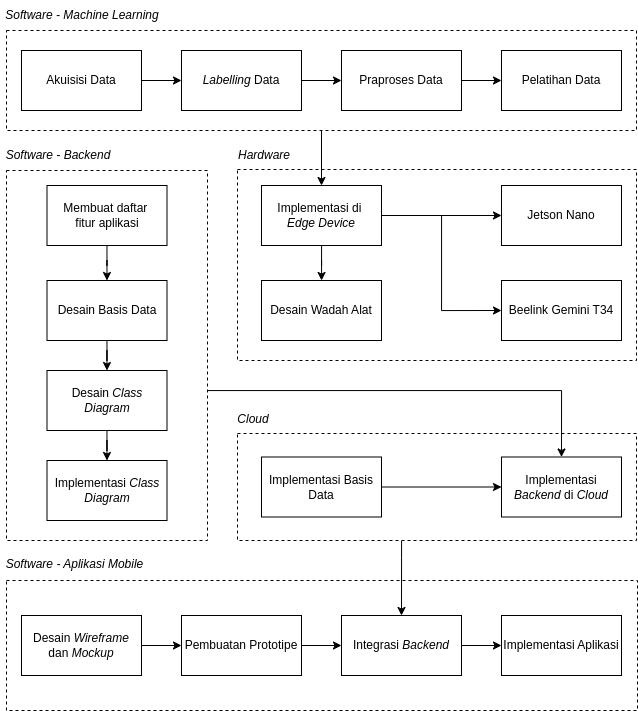
\includegraphics[scale=0.55]{gambar/bab3-block-diagram.png}

  \caption{Blok Diagram Sistem Deteksi Kendaraan \emph{Overdimension}}
  \label{fig:blockdiagrammethod}
\end{figure}

Pada Gambar \ref{fig:blockdiagrammethod}, terdapat blok diagram yang menjelaskan bagian-bagian pengembangan sistem deteksi kendaraan \emph{overdimension} yang terbagi menjadi 3 bagian utama, yaitu \emph{software}, \emph{cloud}, \emph{hardware}. Lalu bagian \emph{software} sendiri terbagi menjadi 3 bagian, yaitu \emph{machine learning}, \emph{backend}, dan aplikasi \emph{mobile}. Berikut adalah penjelasan dari masing-masing bagian blok diagram:

\subsection{\emph{Software - Machine Learning}}
Pada bagian ini, dilakukan beberapa tahapan, yaitu:
\begin{enumerate}[nolistsep]
  \item Akuisisi data
  \item \emph{Labelling} data
  \item Praproses data
  \item Pelatihan data
\end{enumerate}

\textbf{Akuisisi data} dilakukan dengan mengambil data video dari kendaraan yang melintas. Akuisisi data dilakukan sebanyak 2 kali, yaitu di Jalan Tanjung Perak dan di Gerbang Tol Dupak 2 setelah memperoleh izin ke Dinas Perhubungan selaku pihak yang menangani pelanggaran \emph{overdimension} dan PT. Jasa Marga selaku pengelola jalan tol. Data video yang diambil nantinya akan dipotong-potong menjadi beberapa \emph{frame}. \emph{Frame-frame} tersebut akan digunakan sebagai data latih untuk model \emph{machine learning} setelah melewati proses \emph{Labelling}. Gambar \ref{fig:acquisitiondata} menunjukkan proses akuisisi data yang telah dilakukan.

\begin{figure}[htbp]
  \centering
  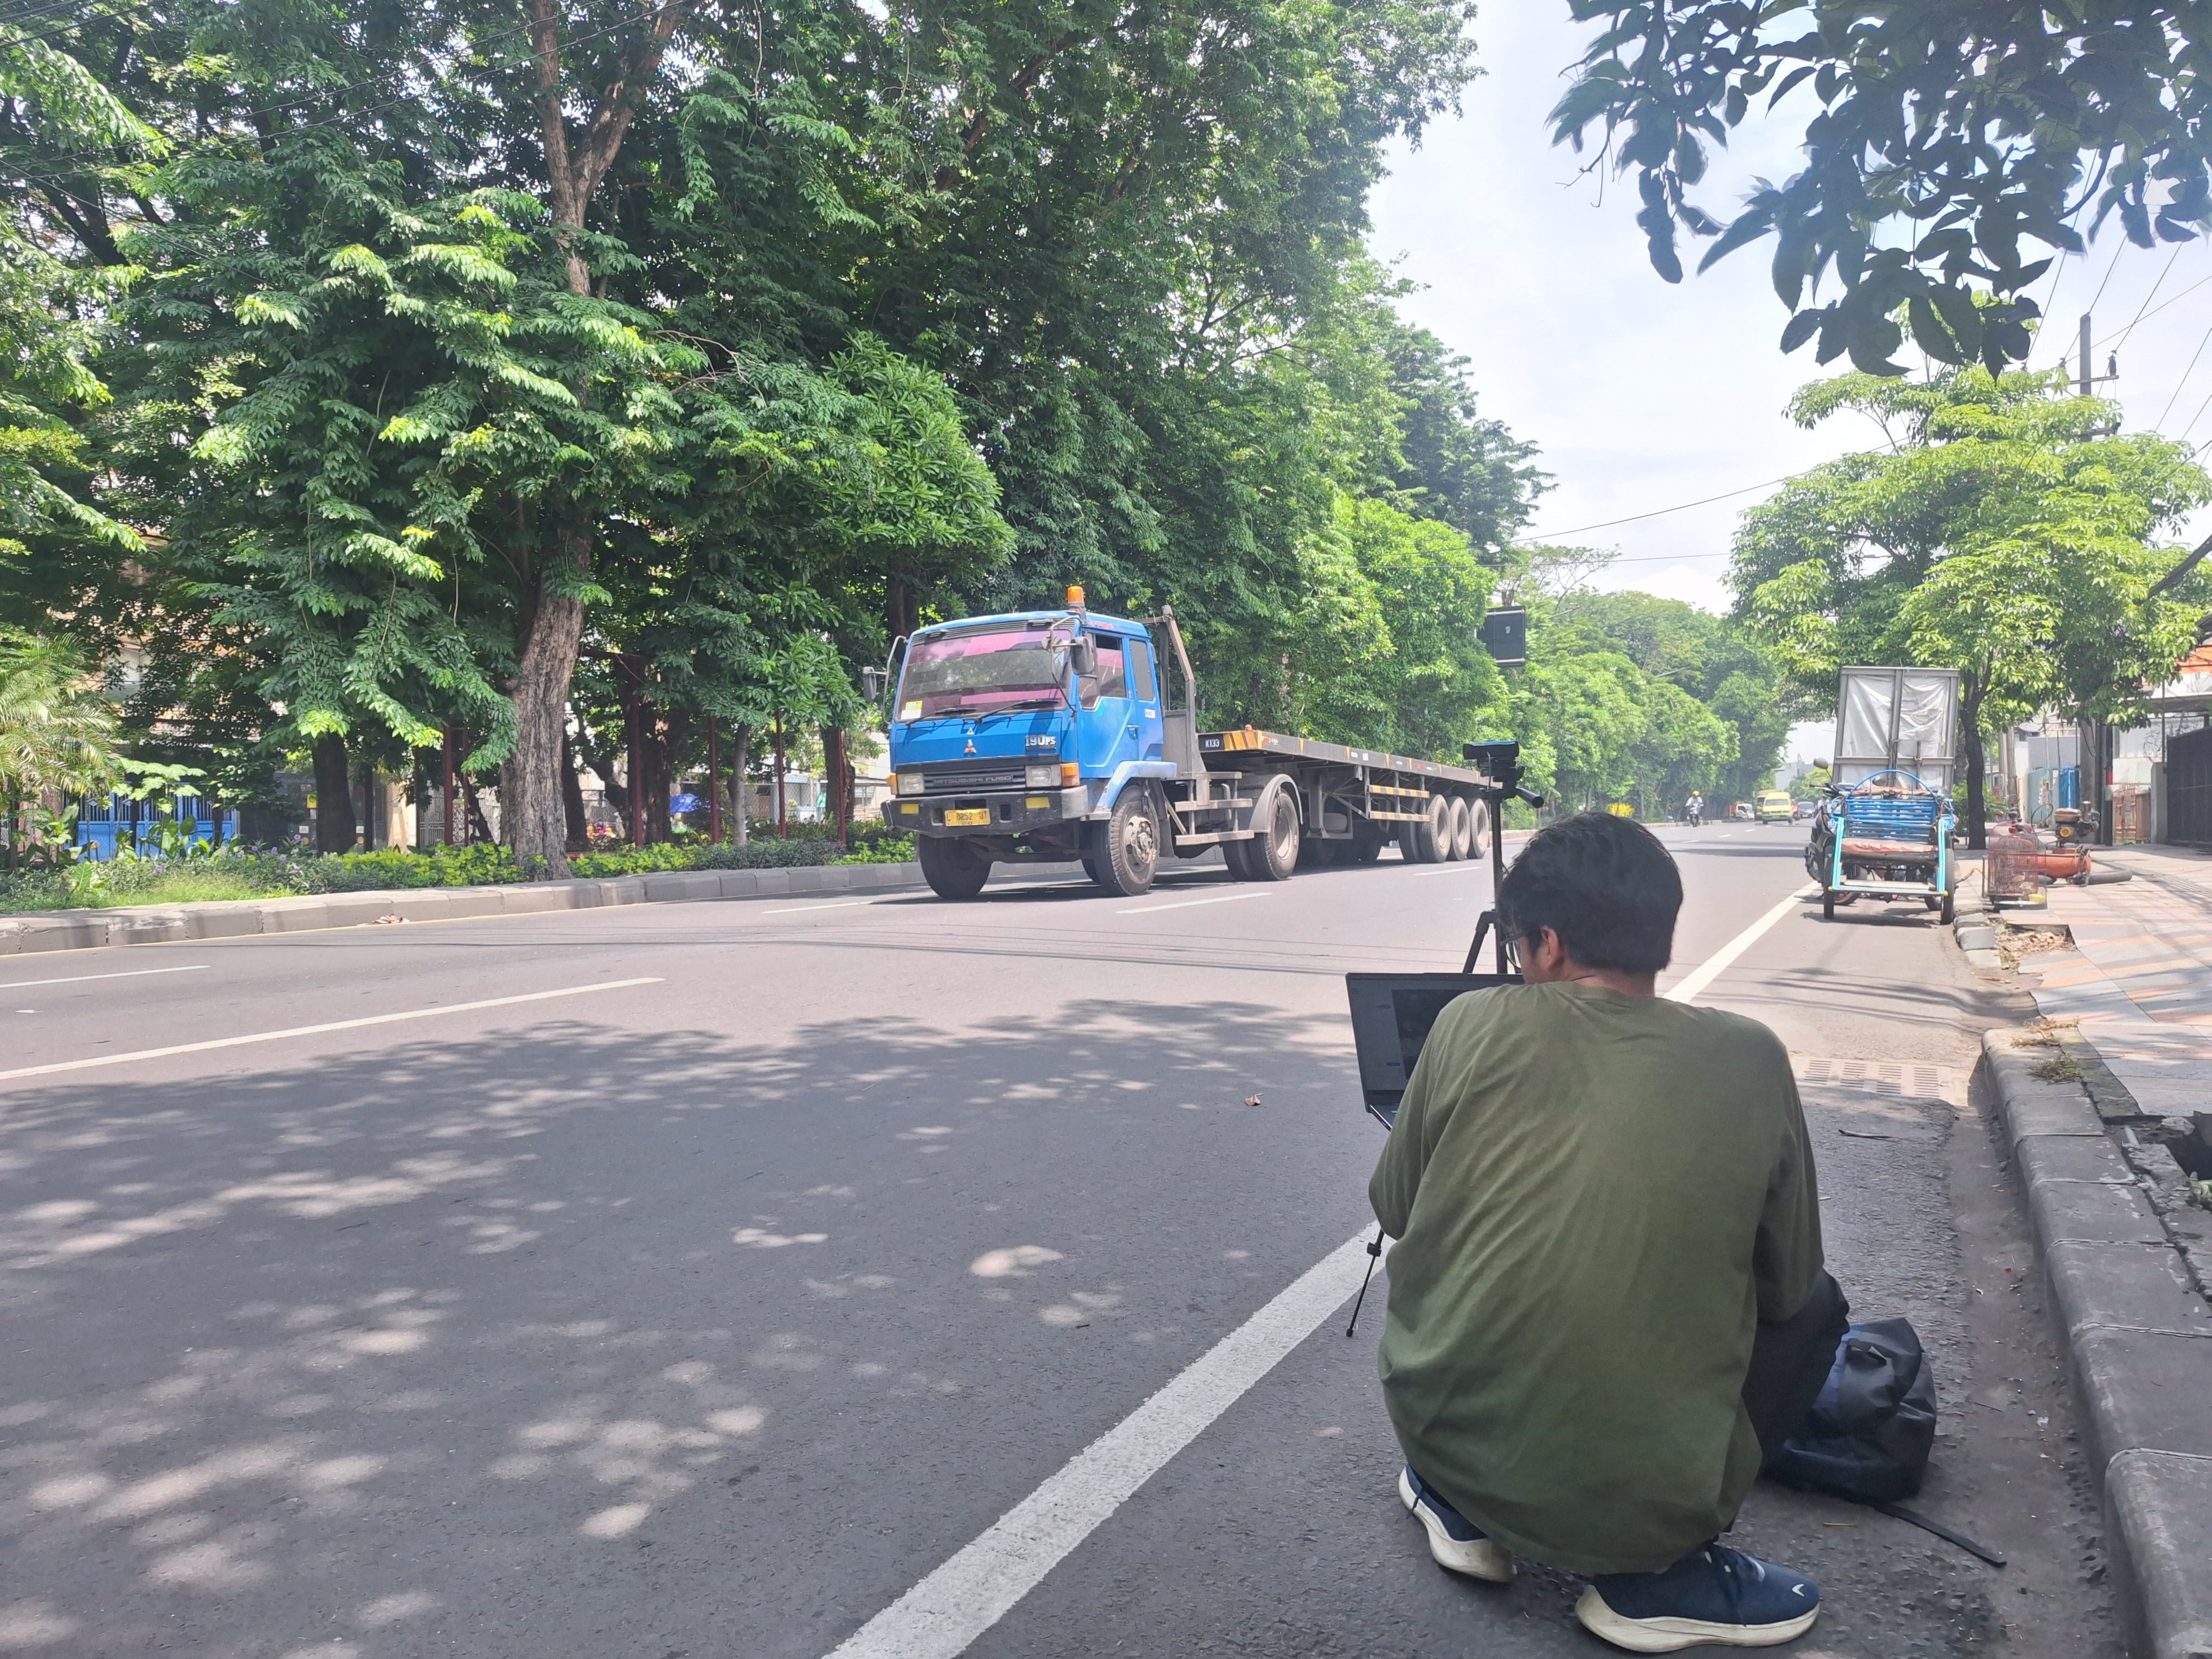
\includegraphics[scale=0.07]{gambar/bab3-acquisition-data-perak.png}
  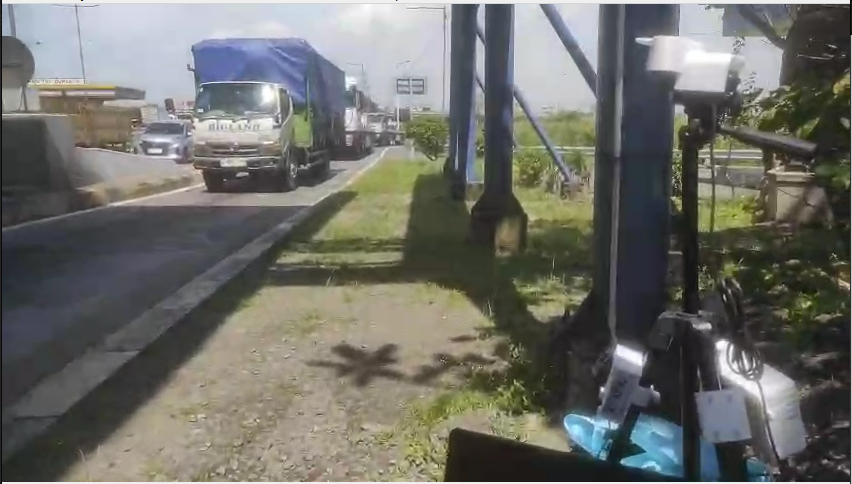
\includegraphics[scale=0.4]{gambar/bab3-acquisition-data-dupak.png}
  \caption{Proses Akuisisi Data, (atas) Jalan Tanjung Perak, (bawah) Gerbang Tol Dupak 2}
  \label{fig:acquisitiondata}
\end{figure}

\textbf{\emph{Labelling} data} dilakukan dengan memberikan label pada data yang telah diakuisisi. Label yang diberikan adalah jenis kendaraan yang melintas dan apakah kendaraan tersebut termasuk \emph{overdimension} atau tidak. Proses \emph{labelling} ini dilakukan dengan menggunakan aplikasi \emph{Roboflow}. Gambar \ref{fig:labellingdata} menunjukkan proses \emph{labelling} data yang telah dilakukan.

\begin{figure}[htbp]
  \centering

  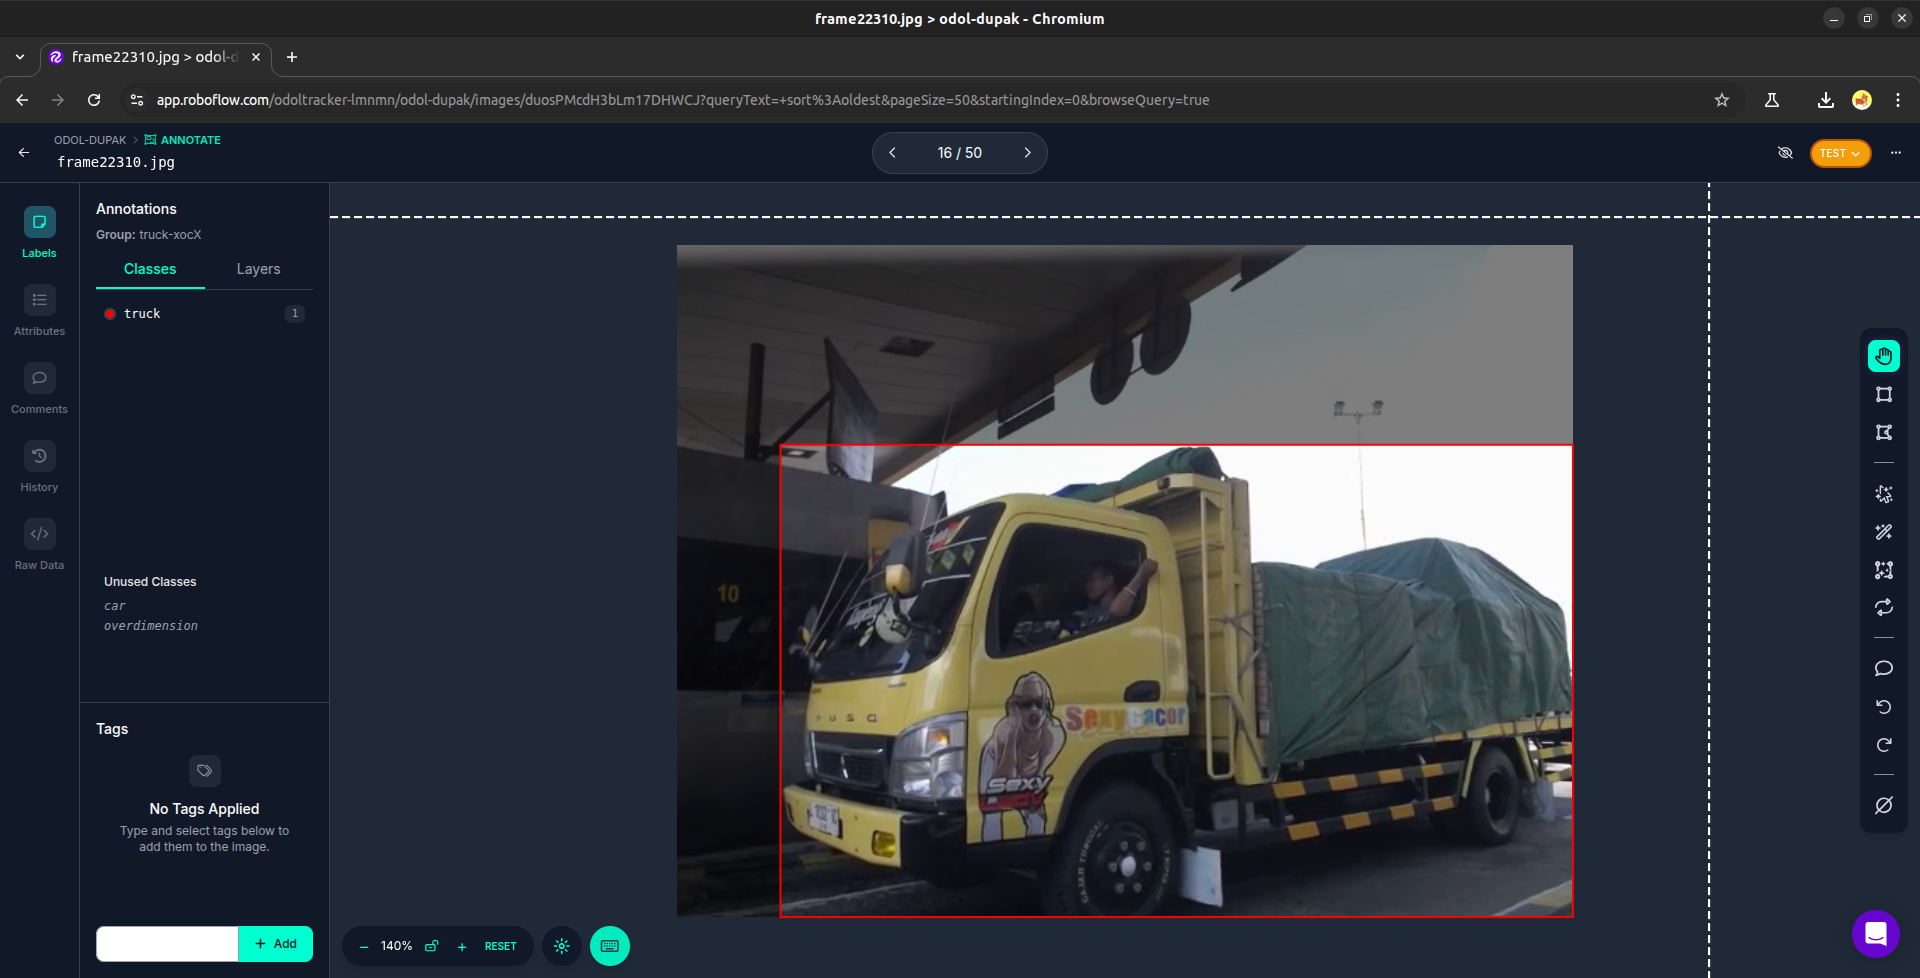
\includegraphics[scale=0.2]{gambar/bab3-labelling-data-nonoverdimension.png}
  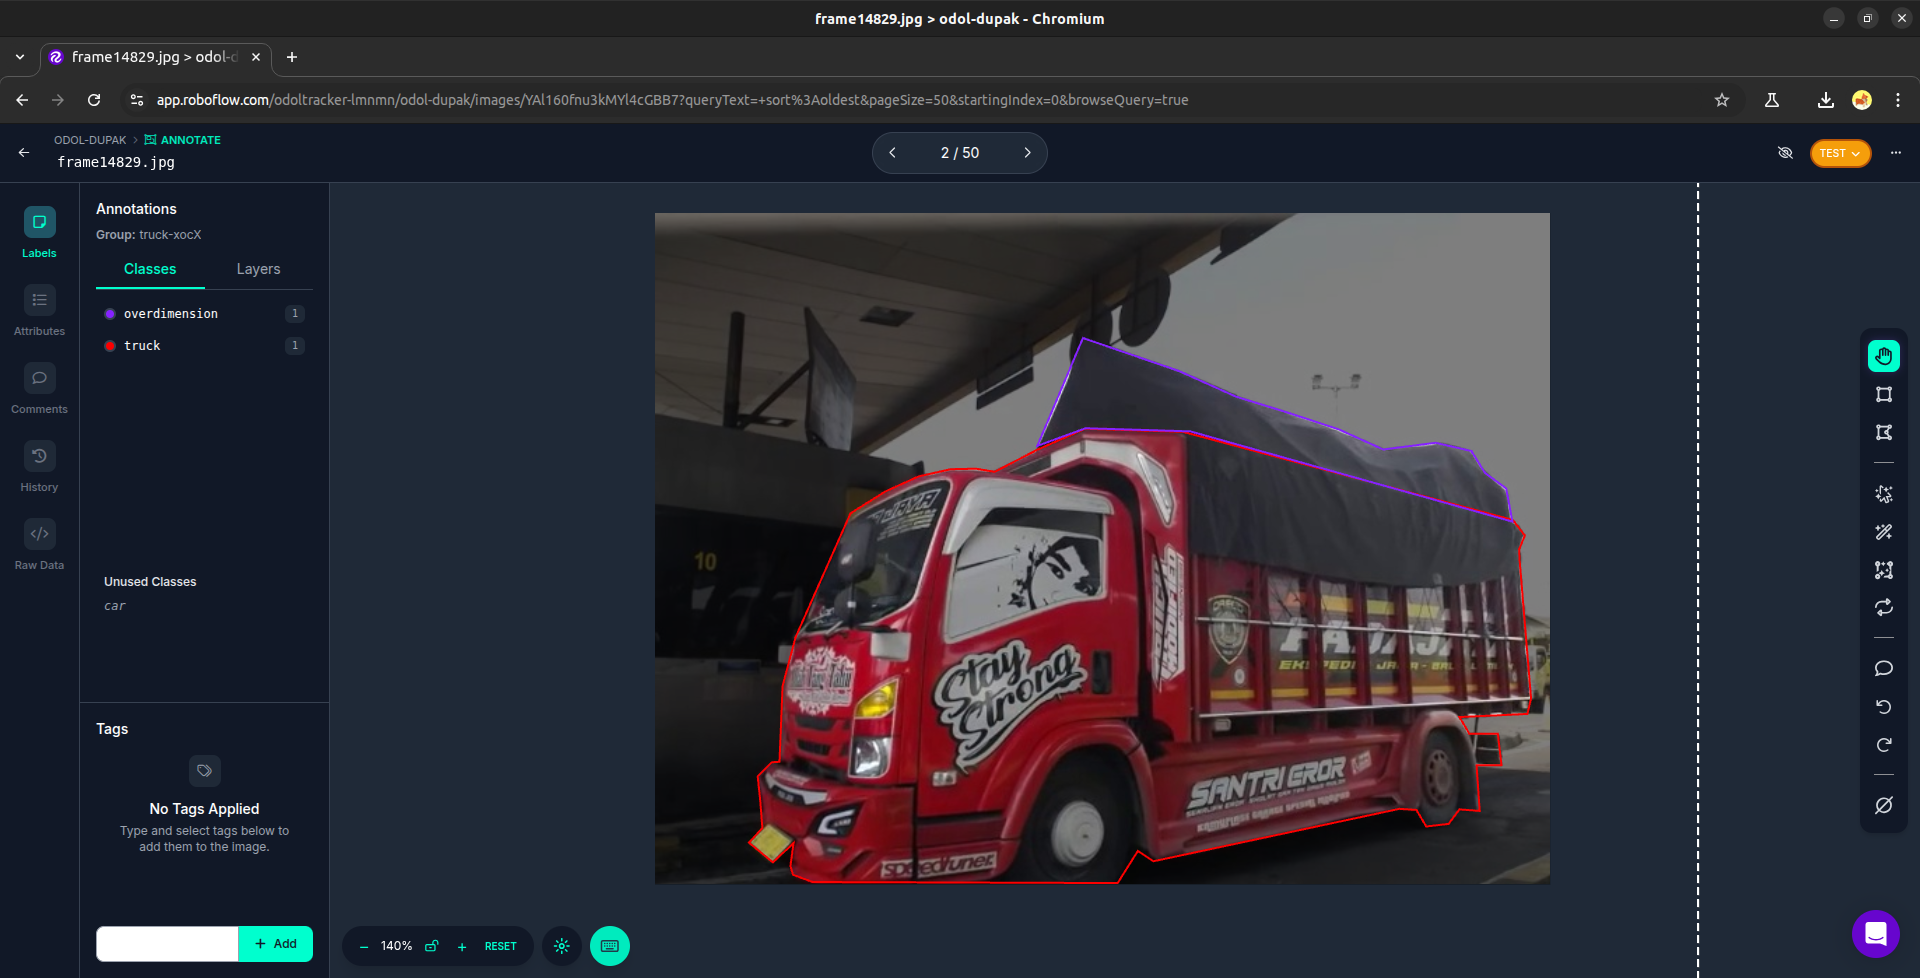
\includegraphics[scale=0.2]{gambar/bab3-labelling-data-overdimension.png}

  \caption{\centering Proses \emph{Labelling} data menggunakan aplikasi \emph{Roboflow}, (atas) Kendaraan Non-\emph{Overdimension}, (bawah) Kendaraan \emph{Overdimension}}
  \label{fig:labellingdata}
\end{figure}

Di penelitian ini, kendaraan yang overdimension diberikan label \emph{truck} dan \emph{overdimension} pada muatannya menggunakan \emph{polygon}. Sedangkan kendaraan yang non-overdimension diberikan label \emph{car} (agar model tidak salah mengklasifikasikan truk sebagai mobil) dengan \emph{bounding box} biasa. Ilustrasi dari \emph{labelling} data dapat dilihat pada Gambar \ref{fig:labellingdataillustration}.

\begin{figure}[htbp]
  \centering
  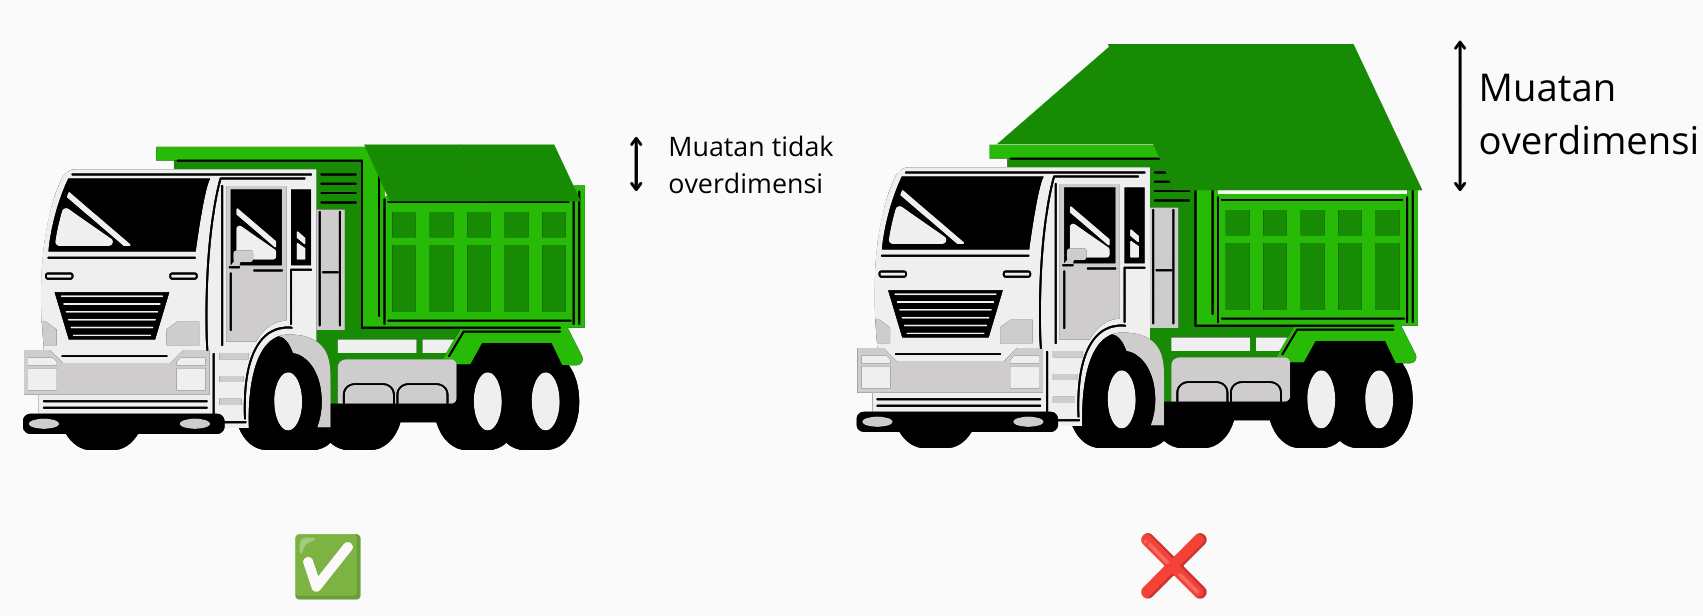
\includegraphics[scale=0.25]{gambar/bab3-truck-detection-method.png}

  \caption{\centering Ilustrasi \emph{Labelling} data, (kiri) Kendaraan Non-\emph{Overdimension}, (kanan) Kendaraan \emph{Overdimension}}
  \label{fig:labellingdataillustration}
\end{figure}

\textbf{Praproses data} dilakukan setelah data telah diberi label. Hal ini bertujuan untuk mempersiapkan data yang akan digunakan sebagai data latih pada model \emph{machine learning} dalam hal ini SSD-MobileNetV2. Pada awalnya data yang telah diberi label akan disesuaikan orientasinya dan di-\emph{resize} ke ukuran 300x300 piksel. Kemudian dilakukan juga augmentasi data dengan cara memberikan \emph{brightness} (kecerahan) sebanyak -12\% hingga 12\% dan \emph{exposure} (paparan) sebanyak -10\% hingga 10\%.

Setelah itu, data akan dibagi menjadi data latih dan data validasi dengan perbandingan 80:20. Gambar \ref{fig:citraasli} menunjukkan citra asli yang akan dipraproses, sedangkan Gambar \ref{fig:preprocessingdata} menunjukkan proses praproses data yang telah dilakukan.

\begin{figure}[htbp]
  \centering

  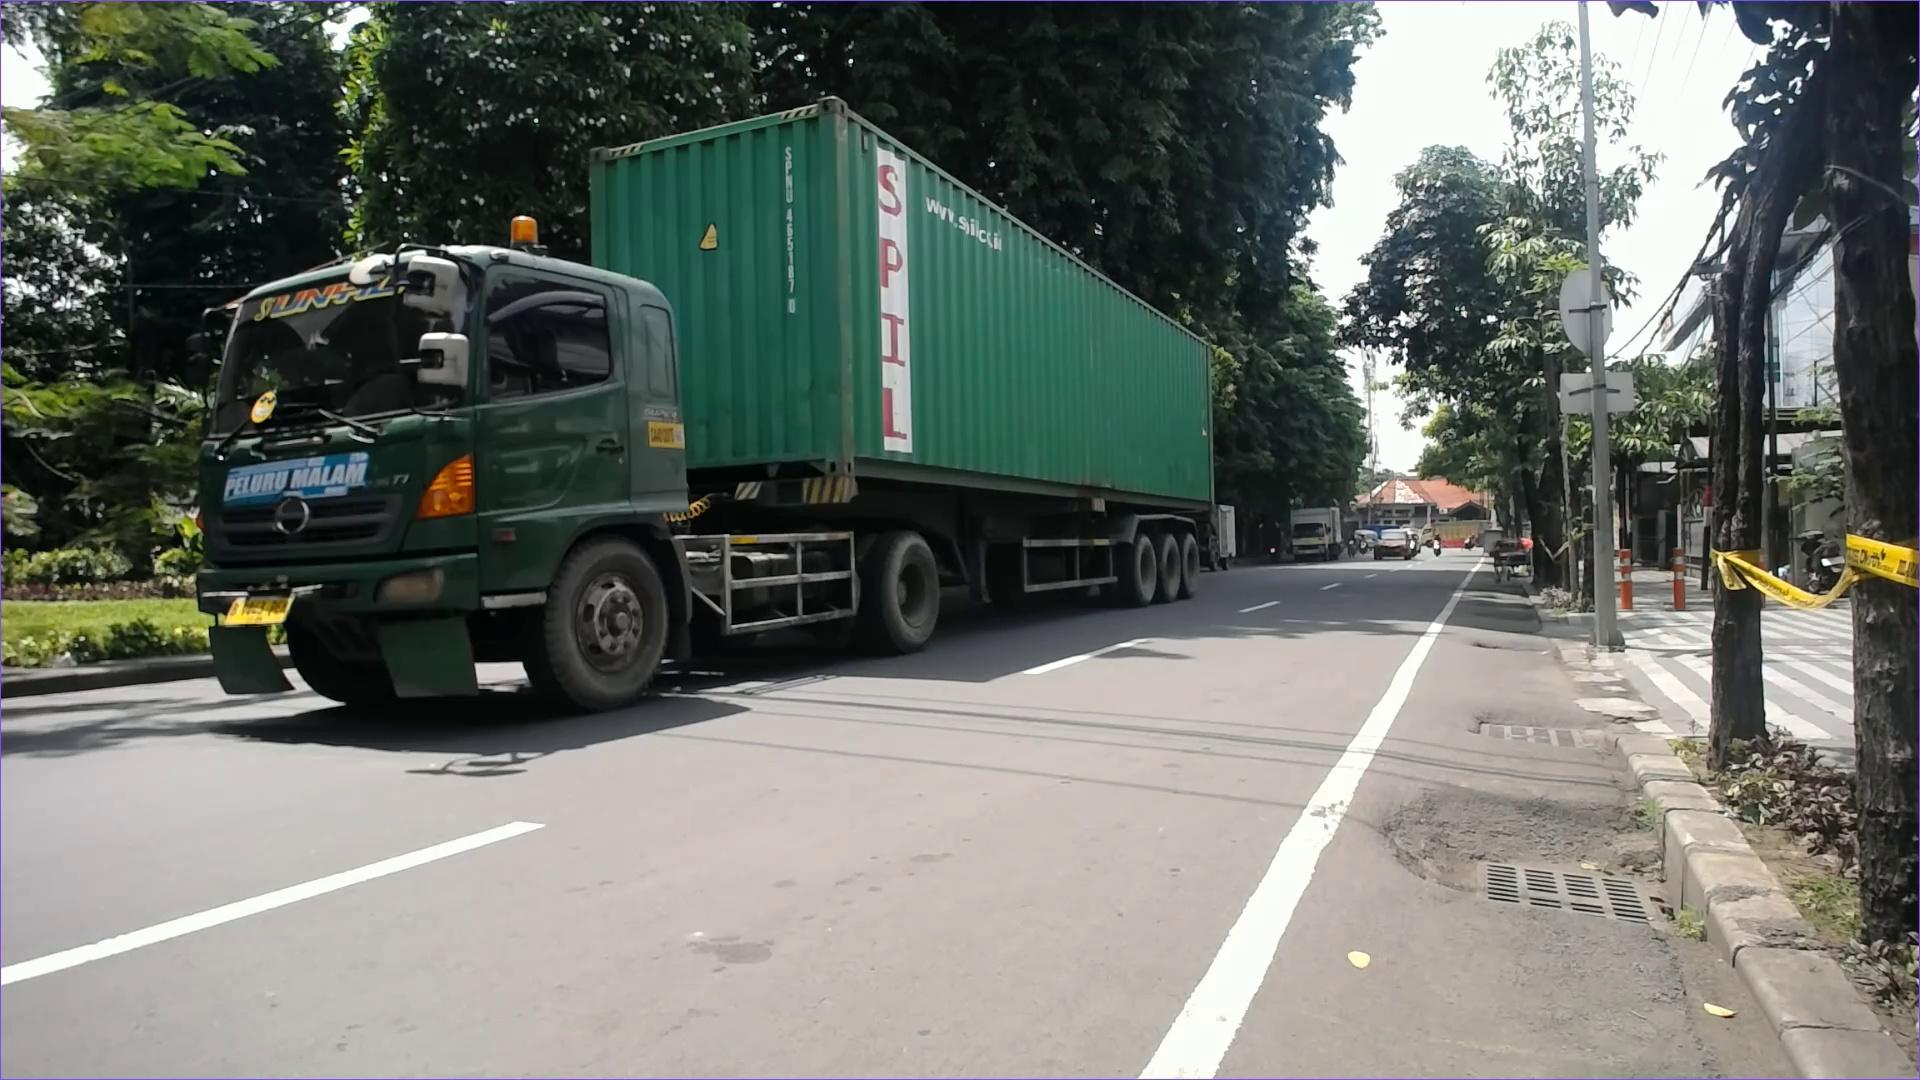
\includegraphics[scale=0.5]{gambar/bab3-citra-asli.jpg}
  \caption{Data citra sebelum dilakukan praproses}
  \label{fig:citraasli}
  
\end{figure}

\begin{figure}[htbp]
  \centering

  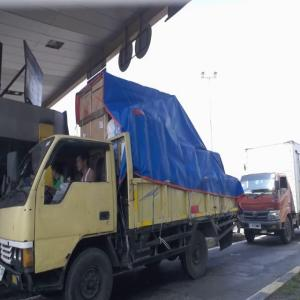
\includegraphics[scale=0.45]{gambar/bab3-citra-300x300.jpg}
  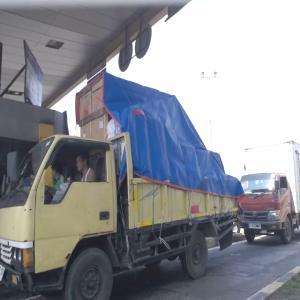
\includegraphics[scale=0.45]{gambar/bab3-citra-300x300-brightness-up.jpg}
  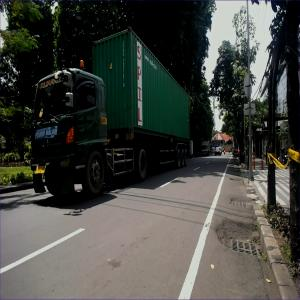
\includegraphics[scale=0.45]{gambar/bab3-citra-300x300-brightness-down.jpg}

  \caption{\centering Data citra setelah dilakukan praproses, (kiri) setelah di-\emph{resize} ke ukuran 300x300, (tengah) citra 300x300 dengan kecerahan dan paparan naik, (kanan) citra 300x300 dengan kecerahan dan paparan turun}
  \label{fig:preprocessingdata}
\end{figure}

\textbf{Pelatihan data} dilakukan setelah data telah dipersiapkan. Data latih yang telah disiapkan akan digunakan untuk melatih model \emph{machine learning} dengan menggunakan \emph{framework} PyTorch. Model yang digunakan adalah SSD-MobileNetV2 yang telah dilatih sebelumnya (\emph{pre-trained model}) dengan menggunakan dataset COCO. Proses pelatihan ini akan menghasilkan model yang dapat digunakan untuk mendeteksi kendaraan \emph{overdimension}.

\subsection{\emph{Hardware}}

Pada bagian ini, dilakukan beberapa tahapan, yaitu:
\begin{enumerate}[nolistsep]
  \item Implementasi hasil pelatihan di \emph{Edge Device} di:
  \begin{enumerate}[nolistsep]
    \item Jetson Nano, dan
    \item Beelink Gemini T34
  \end{enumerate} 
  \item Desain dan pencetakan wadah alat
\end{enumerate}

\textbf{Implementasi hasil pelatihan di \emph{Edge Device}} dilakukan setelah model \emph{machine learning} dilatih. Model yang telah dilatih akan diimplementasikan di \emph{Edge Device} yang telah disiapkan, yaitu Jetson Nano dan Beelink Gemini T34. Implementasi ini bertujuan untuk mendeteksi kendaraan \emph{overdimension} secara \emph{real-time} dan mengintegrasikan hasil deteksi dengan sistem yang ada. Gambar \ref{fig:implementationedgedevice} menunjukkan hasil implementasi model \emph{machine learning} di \emph{Edge Device} yang telah dilakukan.

\begin{figure}[htbp]
  \centering

  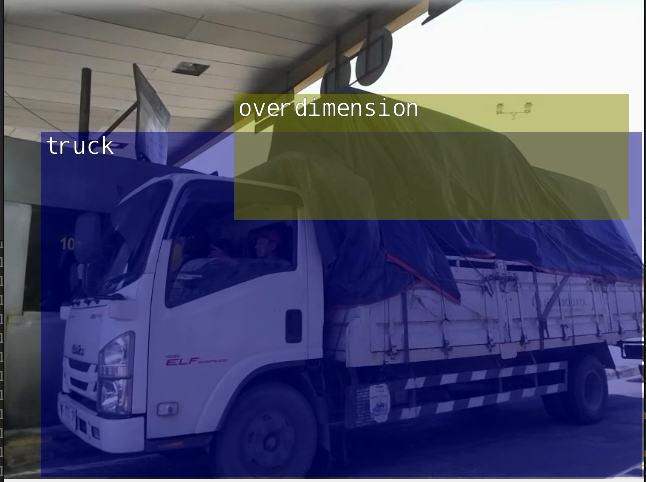
\includegraphics[scale=0.3]{gambar/bab3-implementasi-di-jetson.png}
  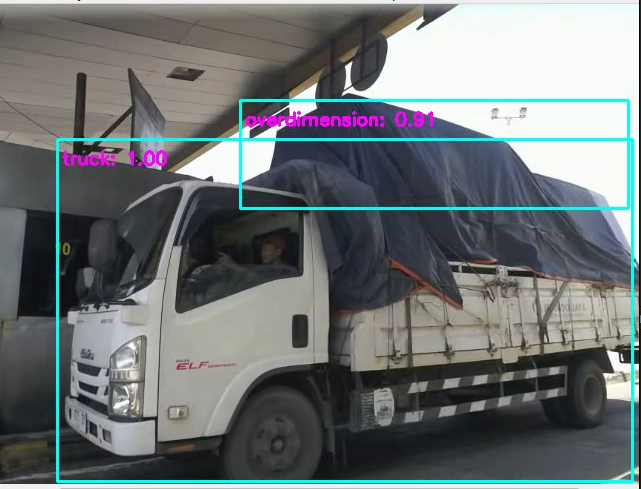
\includegraphics[scale=0.3]{gambar/bab3-implementasi-di-beelink.png}

  \caption{\centering Implementasi Model \emph{Machine Learning} di \emph{Edge Device}, (kiri) Jetson Nano, (kanan) Beelink Gemini T34}
  \label{fig:implementationedgedevice}
\end{figure}

\textbf{Desain dan pencetakan wadah alat} dilakukan setelah model \emph{machine learning} berhasil diimplementasikan di \emph{Edge Device}. Wadah alat ini berfungsi sebagai tempat untuk meletakkan \emph{Edge Device} dan kamera yang digunakan untuk mendeteksi kendaraan \emph{overdimension}. Gambar \ref{fig:designcontainercamera} dan \ref{fig:designcontainerjetson} masing-masing menunjukkan desain wadah kamera dan wadah Jetson Nano yang telah dibuat. Untuk Beelink Gemini T34, setelah dilakukan pengujian lebih lanjut, ditemukan bahwa perangkat ini memiliki keterbatasan dalam melakukan inferensi model secara \emph{real-time} karena hanya mengandalkan CPU. Meskipun telah dilakukan optimasi, performa inferensi tetap tidak memadai untuk aplikasi deteksi \emph{real-time}, sehingga pengembangan wadah khusus untuk perangkat ini tidak dilanjutkan.

\begin{figure}[htbp]
  \centering

  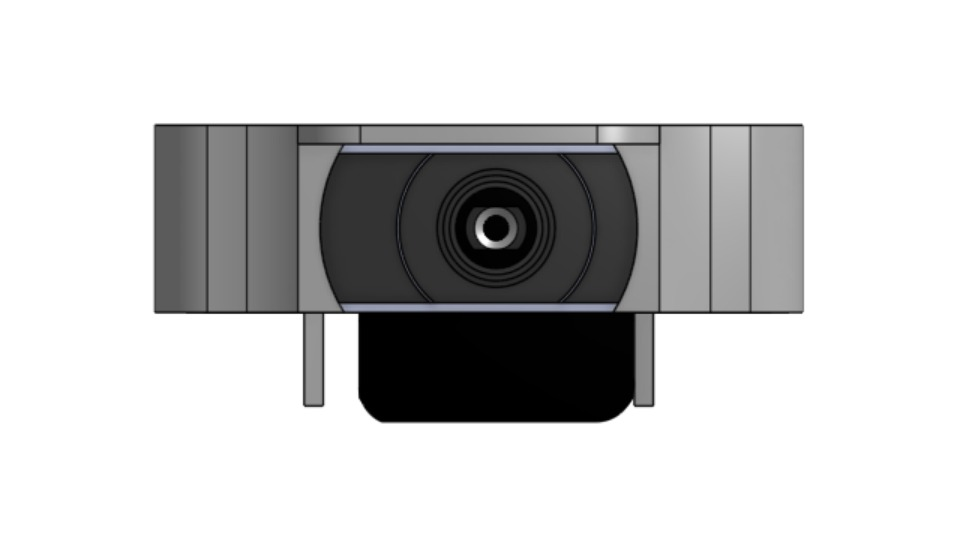
\includegraphics[scale=0.16]{gambar/bab3-tampak-depan-case-camera.jpeg}
  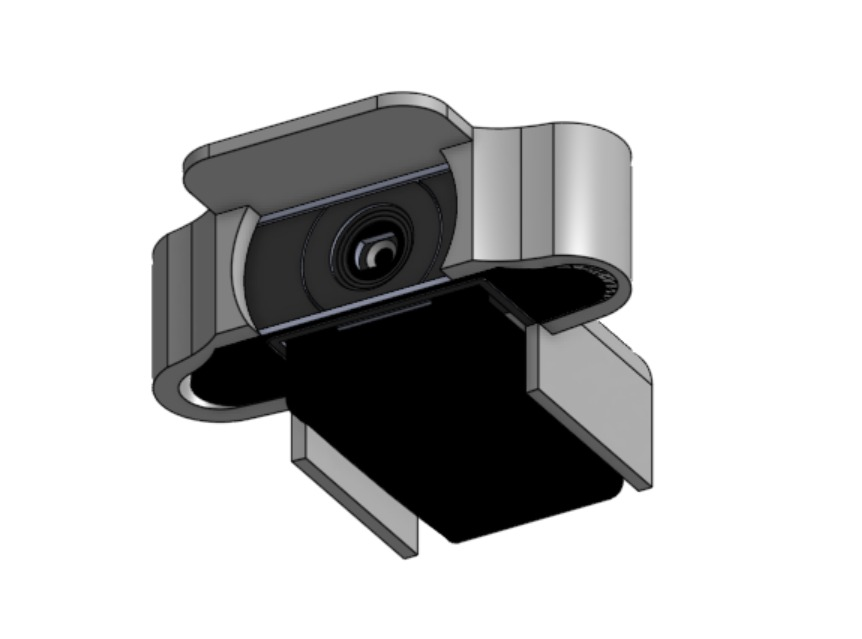
\includegraphics[scale=0.16]{gambar/bab3-tampak-samping-case-camera.jpeg}
  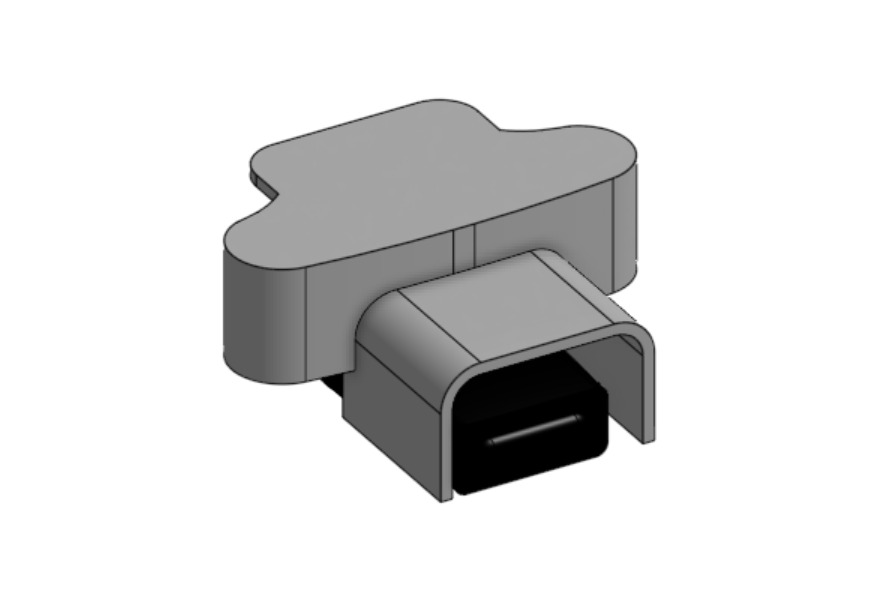
\includegraphics[scale=0.16]{gambar/bab3-tampak-belakang-case-camera.jpeg}

  \caption{\centering Desain Wadah Kamera, (kiri) Tampak Depan, (tengah) Tampak Samping, (kanan) Tampak Belakang}
  \label{fig:designcontainercamera}
\end{figure}

\begin{figure}[htbp]
  \centering

  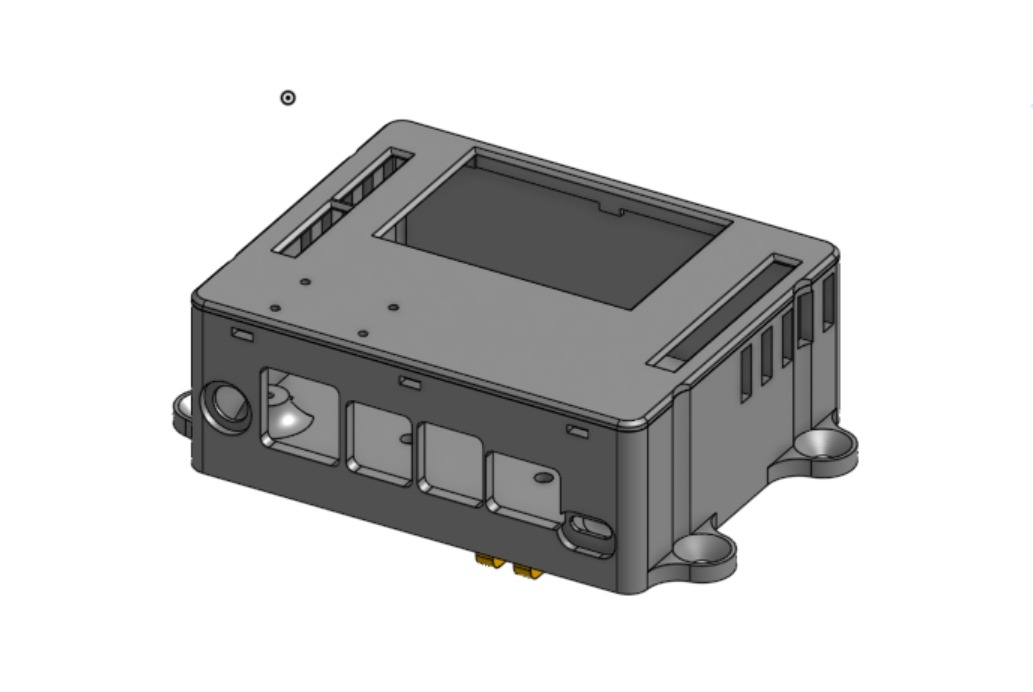
\includegraphics[scale=0.13]{gambar/bab3-tampak-depan-case-jnano.jpeg}
  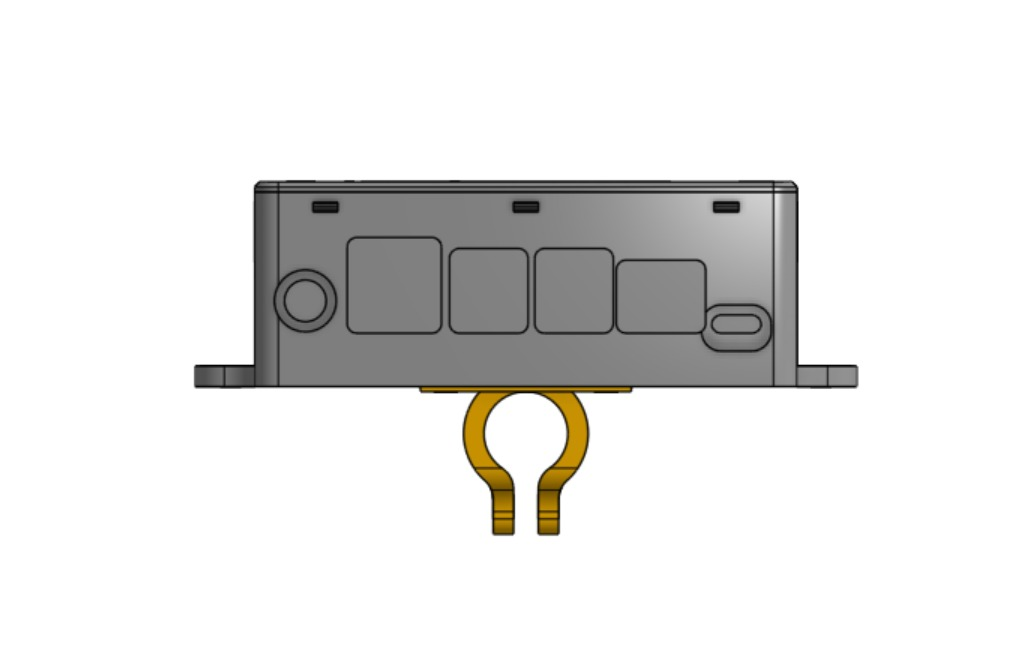
\includegraphics[scale=0.13]{gambar/bab3-tampak-samping-case-jnano.jpeg}
  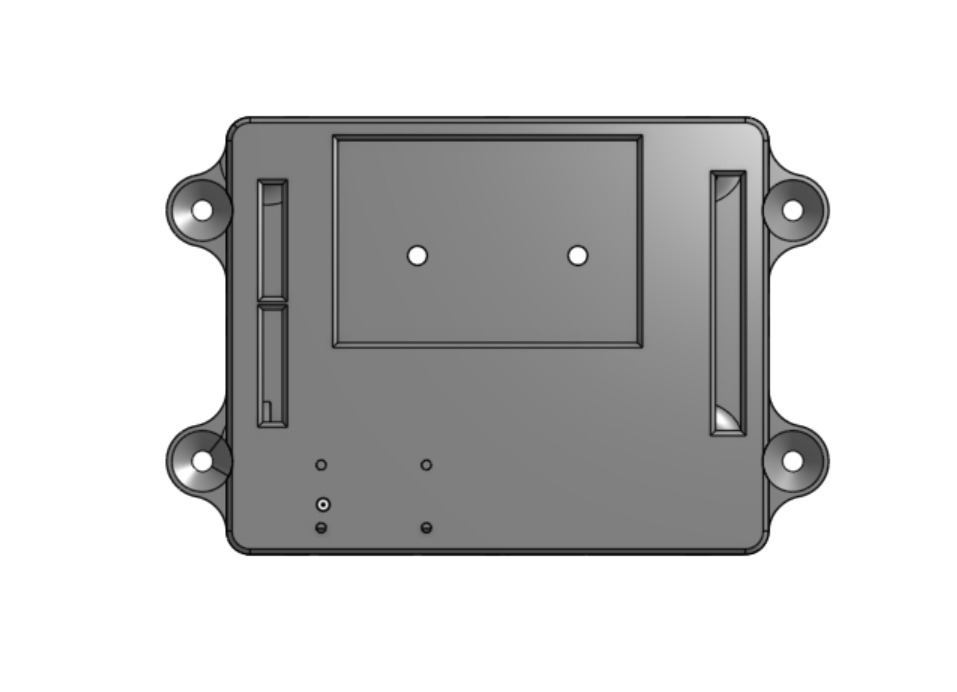
\includegraphics[scale=0.13]{gambar/bab3-tampak-bawah-case-jnano.jpeg}

  \caption{\centering Desain Wadah Jetson Nano, (kiri) Tampak Depan, (tengah) Tampak Samping, (kanan) Tampak Bawah}
  \label{fig:designcontainerjetson}
\end{figure}

Setelah didesain, wadah alat tersebut kemudian dicetak menggunakan printer 3D. Gambar \ref{fig:printcontainer} masing-masing menunjukkan hasil pencetakan wadah kamera dan wadah Jetson Nano.

\begin{figure}[htbp]
  \centering

  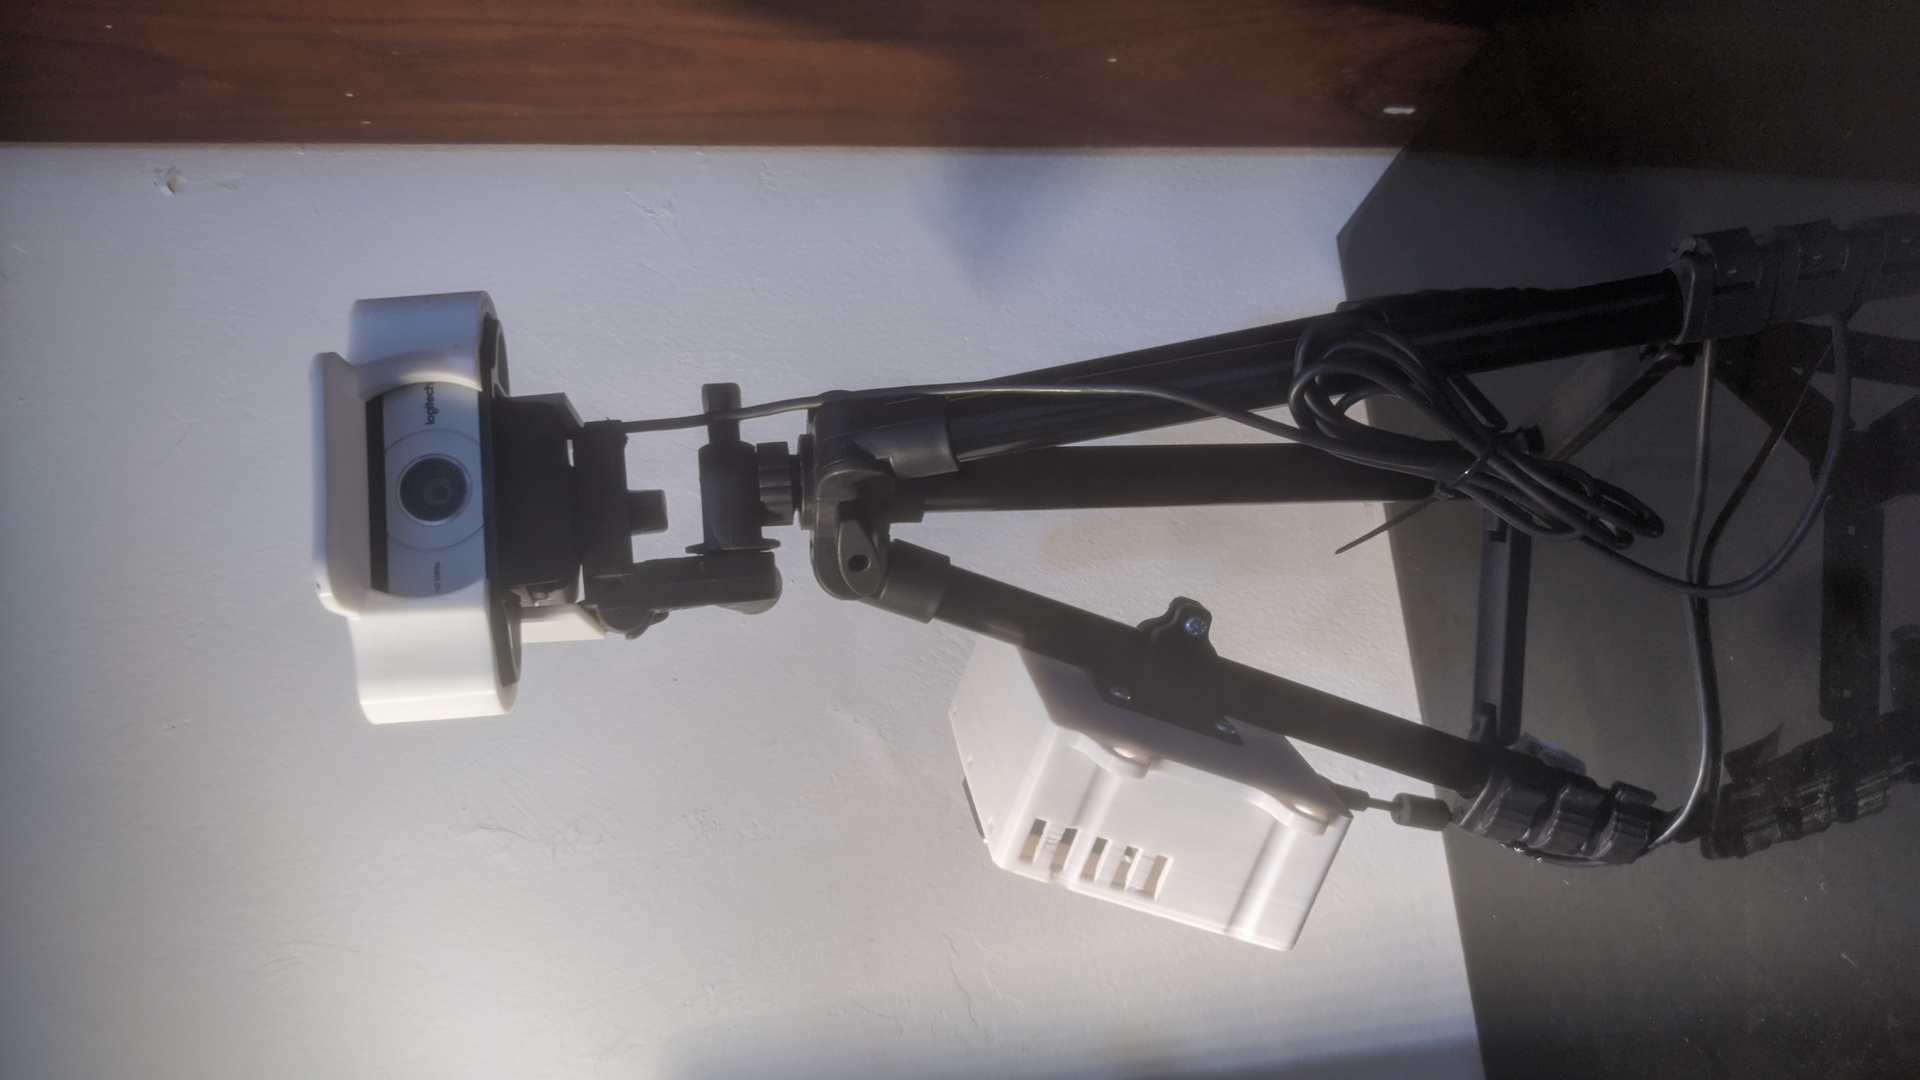
\includegraphics[scale=0.15,angle=-90]{gambar/bab3-case-camera-printed.jpg}
  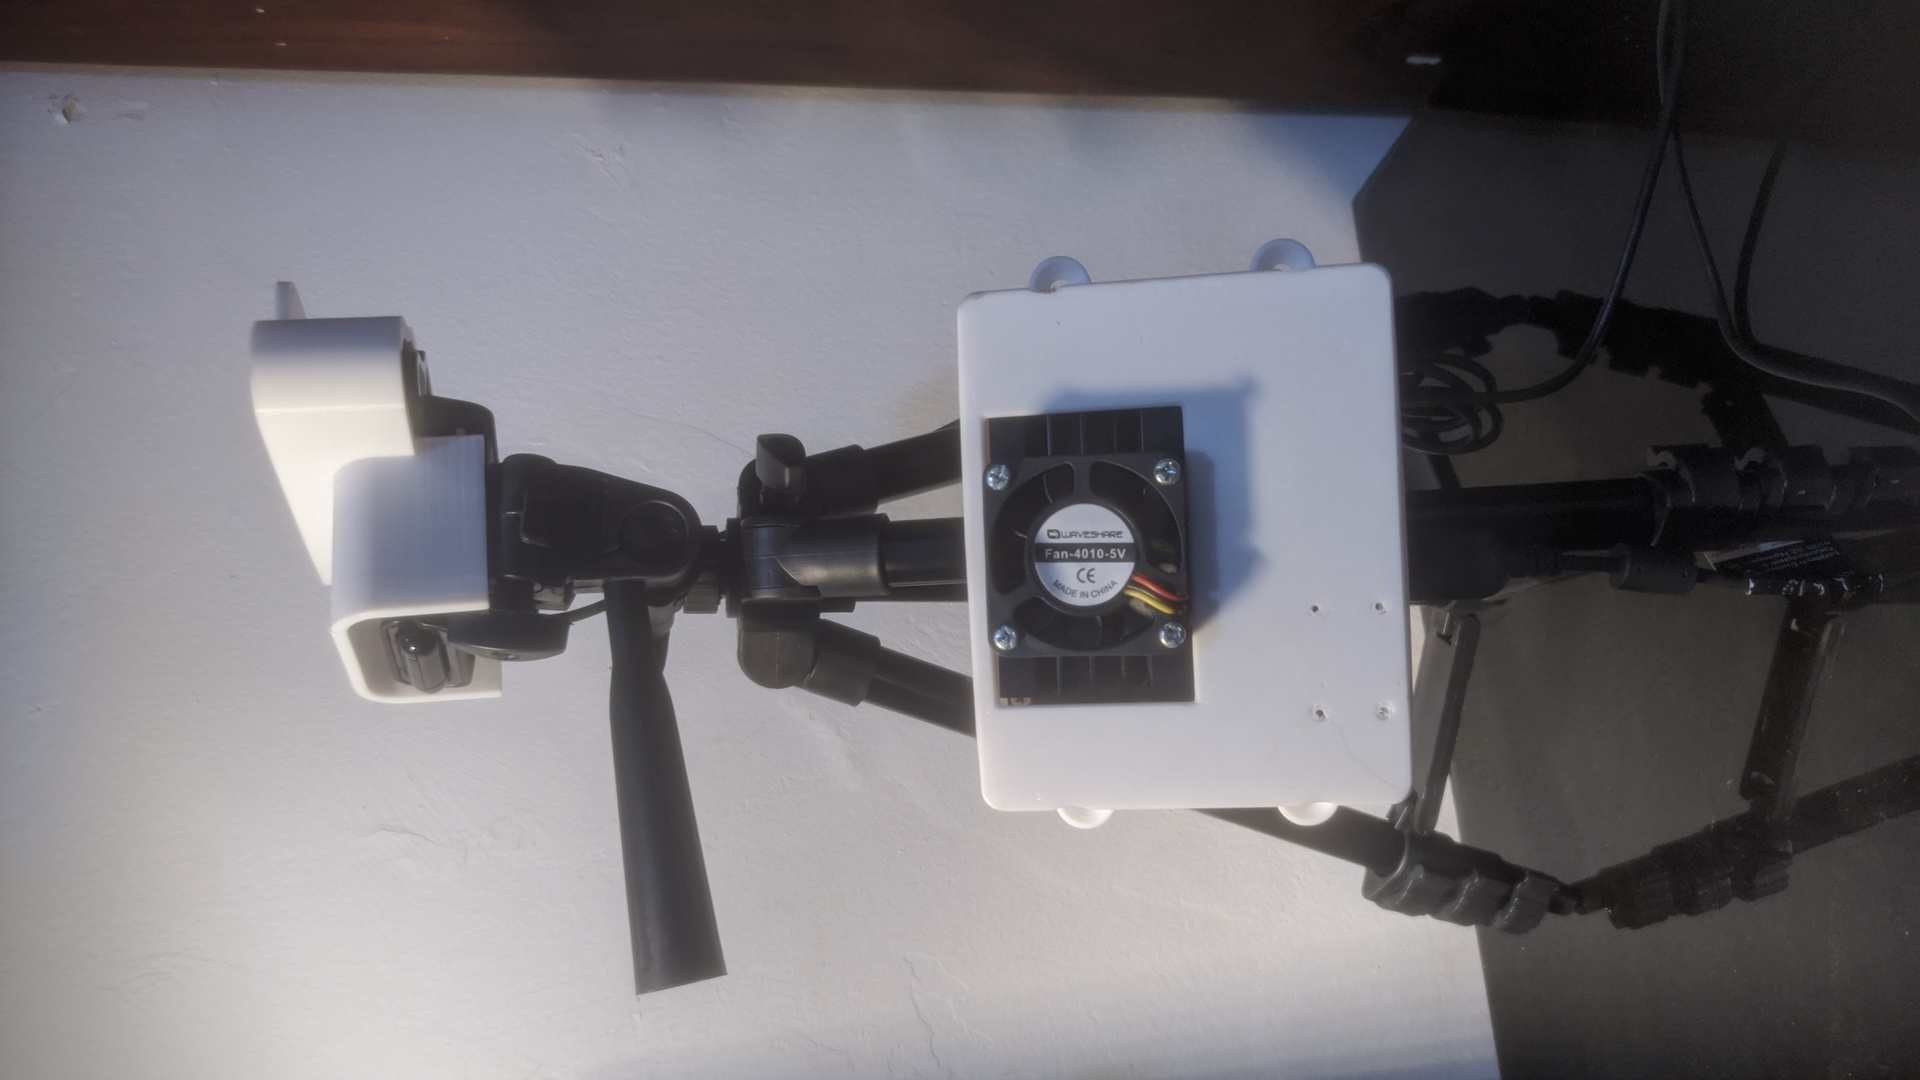
\includegraphics[scale=0.15,angle=-90]{gambar/bab3-case-jnano-printed.jpg}

  \caption{\centering Hasil pencetakan wadah, (kiri) Wadah Kamera, (kanan) Wadah Jetson Nano}
  \label{fig:printcontainer}
\end{figure}

\subsection{\emph{Software - Backend}}

Pada bagian ini, dilakukan beberapa tahapan, yaitu:
\begin{enumerate}[nolistsep]
  \item Membuat daftar fitur aplikasi
  \item Desain basis data
  \item Desain \emph{class diagram}
  \item Implementasi \emph{class diagram}
\end{enumerate}

\textbf{Membuat daftar fitur aplikasi} dilakukan untuk menentukan fitur-fitur yang akan ada pada aplikasi, sehingga dapat mempermudah desain basis data dan desain \emph{class diagram}. Fitur-fitur yang ada pada aplikasi ini adalah:
\begin{itemize}[nolistsep]
  \item Pendaftaran akun
  \item Login
  \item Dashboard berbeda untuk admin dan operator
  \item Analitik data
  \item Notifikasi
  \item Verifikasi pelanggaran
  \item Edit profil
  \item Ubah kata sandi
  \item Lupa kata sandi
\end{itemize}

Sehingga dapat disimpulkan bahwa aplikasi ini memiliki 2 jenis pengguna, yaitu admin dan operator. Admin memiliki akses penuh terhadap aplikasi, sedangkan operator hanya dapat mengakses fitur-fitur tertentu saja, contohnya operator tidak bisa mendapatkan semua user yang terdaftar di aplikasi sedangkan admin bisa.

\textbf{Desain basis data} dilakukan untuk menentukan struktur basis data yang akan digunakan pada aplikasi. Basis data yang digunakan adalah basis data \emph{relational} dengan menggunakan \emph{PostgreSQL}. Tabel-tabel yang ada pada basis data ini adalah:
\begin{itemize}[nolistsep]
  \item Tabel \emph{Users}
  \item Tabel \emph{TollGates}
  \item Tabel \emph{Notifications}
  \item Tabel \emph{VehicleDetections}
  \item Tabel \emph{Images}
\end{itemize}

Gambar \ref{fig:databasedesign} menunjukkan desain basis data yang telah dibuat menggunakan \emph{website} \emph{dbdiagram.io}. Desain basis data ini menggambarkan relasi antar tabel yang ada pada basis data. Tabel-tabel tersebut memiliki relasi satu sama lain, sehingga dapat saling berhubungan dan mempermudah dalam pengolahan data.
\begin{figure}[htbp]
  \centering

  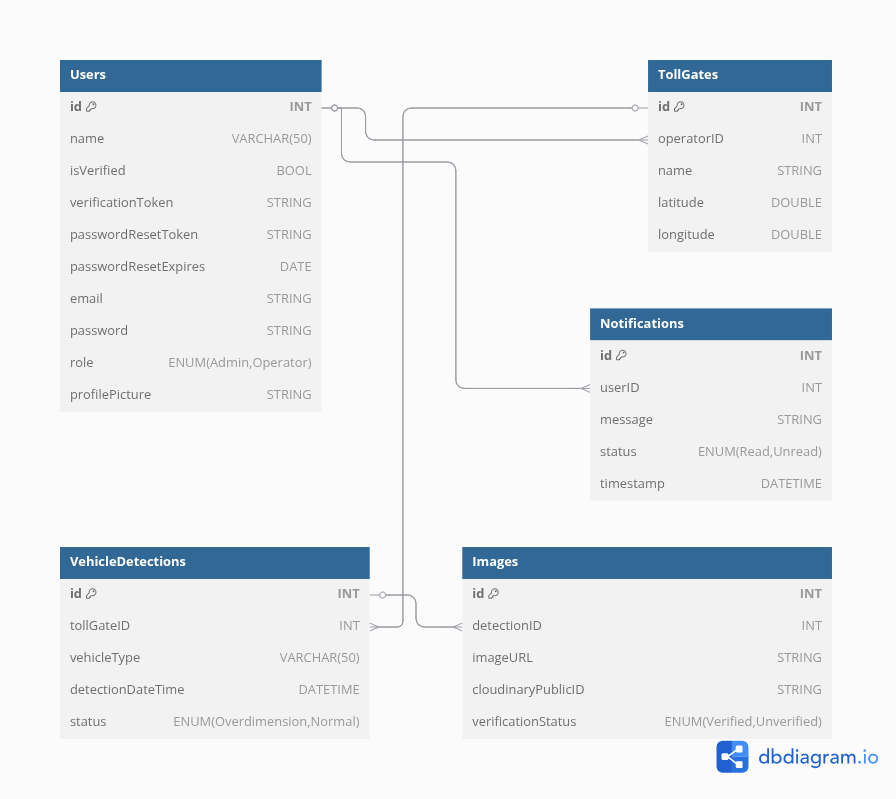
\includegraphics[scale=0.5]{gambar/bab3-desain-database.png}

  \caption{Desain Basis Data}
  \label{fig:databasedesign}
\end{figure}
Dari tabel-tabel yang ada pada basis data tersebut, dapat dilihat bahwa:

\begin{itemize}[nolistsep]
  \item Tabel \emph{Users} berisi data pengguna aplikasi, baik admin maupun operator. Tabel ini memiliki relasi \emph{one to many} dengan tabel \emph{VehicleDetections} dan \emph{Notifications}
  \item Tabel \emph{TollGates} berisi data gerbang tol yang ada. Tabel ini memiliki relasi \emph{one to many} dengan tabel \emph{VehicleDetections}
  \item Tabel \emph{Notifications} berisi data notifikasi yang ada pada aplikasi. Baik notifikasi yang dikirimkan oleh sistem maupun notifikasi yang dikirimkan oleh admin kepada operator.
  \item Tabel \emph{VehicleDetections} berisi data deteksi kendaraan yang ada pada aplikasi. Di tabel inilah dilakukan verifikasi status dari kendaraan, apakah kendaraan tersebut \emph{overdimension} atau tidak. Tabel ini memiliki relasi \emph{one to many} dengan tabel \emph{Images}
  \item Tabel \emph{Images} berisi data gambar kendaraan \emph{overdimension} yang terdeteksi. Gambar tidak disimpan dalam basis data, tetapi hanya menyimpan \emph{link} gambar yang ada pada \emph{cloud storage} Cloudinary.
\end{itemize}

\textbf{Desain \emph{class diagram}} dilakukan untuk menentukan struktur \emph{class} yang akan digunakan pada aplikasi. \emph{Class diagram} ini menggambarkan relasi antar \emph{class} yang ada pada aplikasi. \emph{Class-class} tersebut memiliki relasi satu sama lain, sehingga dapat saling berhubungan dan mempermudah dalam pengolahan data. Gambar \ref{fig:classdiagram} menunjukkan desain \emph{class diagram} yang telah dibuat menggunakan \emph{website} \emph{app.diagrams.net}.

\begin{figure}[htbp]
  \centering

  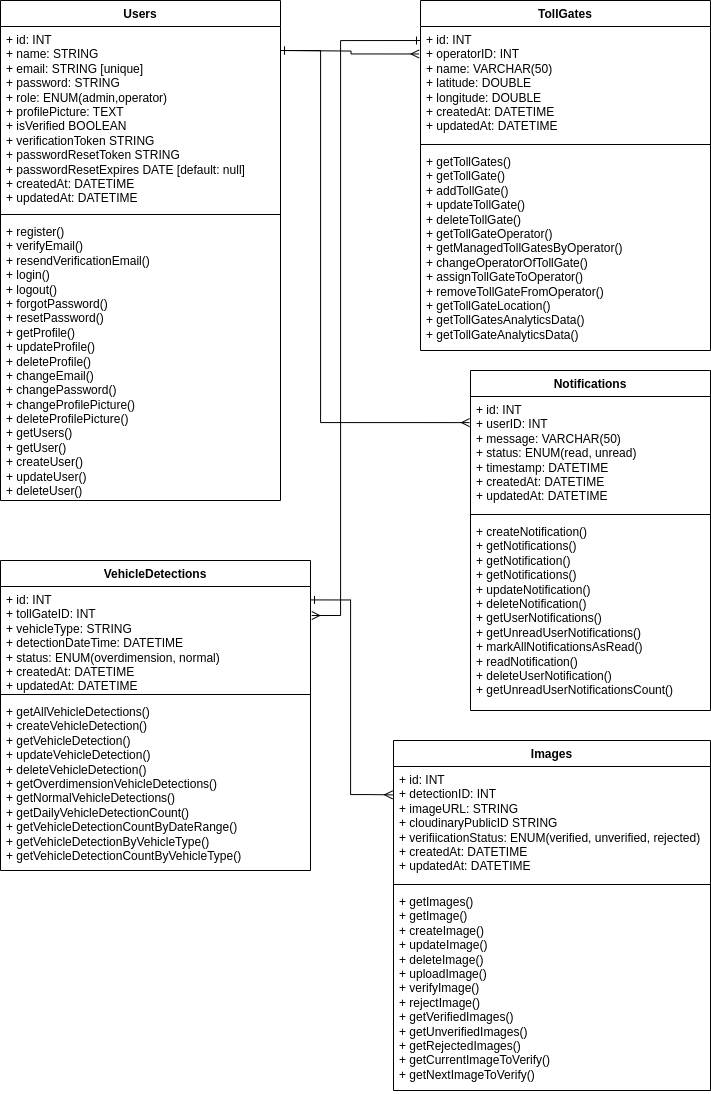
\includegraphics[scale=0.6]{gambar/bab3-class-diagram.png}

  \caption{Desain \emph{Class Diagram}}
  \label{fig:classdiagram}
\end{figure}
Dari \emph{class-class} yang ada pada \emph{class diagram} tersebut, dapat dilihat bahwa:
\begin{itemize}[nolistsep]
  \item Class \emph{User} berisi data pengguna aplikasi, baik admin maupun operator. Class ini memiliki relasi \emph{one to many} dengan class \emph{VehicleDetection} dan \emph{Notification}
  \item Class \emph{TollGate} berisi data gerbang tol yang ada. Class ini memiliki relasi \emph{one to many} dengan class \emph{VehicleDetection}
  \item Class \emph{Notification} berisi data notifikasi yang ada pada aplikasi. Baik notifikasi yang dikirimkan oleh sistem maupun notifikasi yang dikirimkan oleh admin kepada operator.
  \item Class \emph{VehicleDetection} berisi data deteksi kendaraan yang ada pada aplikasi. Di class inilah dilakukan verifikasi status dari kendaraan, apakah kendaraan tersebut \emph{overdimension} atau tidak. Class ini memiliki relasi \emph{one to many} dengan class \emph{Image}
  \item Class \emph{Image} berisi data gambar kendaraan \emph{overdimension} yang terdeteksi. Gambar tidak disimpan dalam basis data, tetapi hanya menyimpan \emph{link} gambar yang ada pada \emph{cloud storage} Cloudinary.
\end{itemize}

\textbf{Implementasi \emph{class diagram}} dilakukan setelah \emph{class diagram} selesai dibuat. \emph{Class-class} yang ada pada \emph{class diagram} akan diimplementasikan ke dalam kode program. Kode program ini ditulis menggunakan bahasa pemrograman JavaScript dengan \emph{framework} Express.js, \emph{ORM} Sequelize, dan \emph{cloud storage} Cloudinary. Kode program ini akan digunakan untuk mengelola data yang ada pada basis data, serta mengelola data yang ada pada \emph{cloud storage} Cloudinary. Setelah \emph{endpoint} selesai dibuat, masing-masing \emph{endpoint} akan di-\emph{test} menggunakan \emph{Postman} untuk memastikan bahwa \emph{endpoint} tersebut dapat berjalan dengan baik. Gambar \ref{fig:implementationclassdiagram} menunjukkan implementasi \emph{class diagram} yang telah dilakukan.

\begin{figure}[htbp]
  \centering

  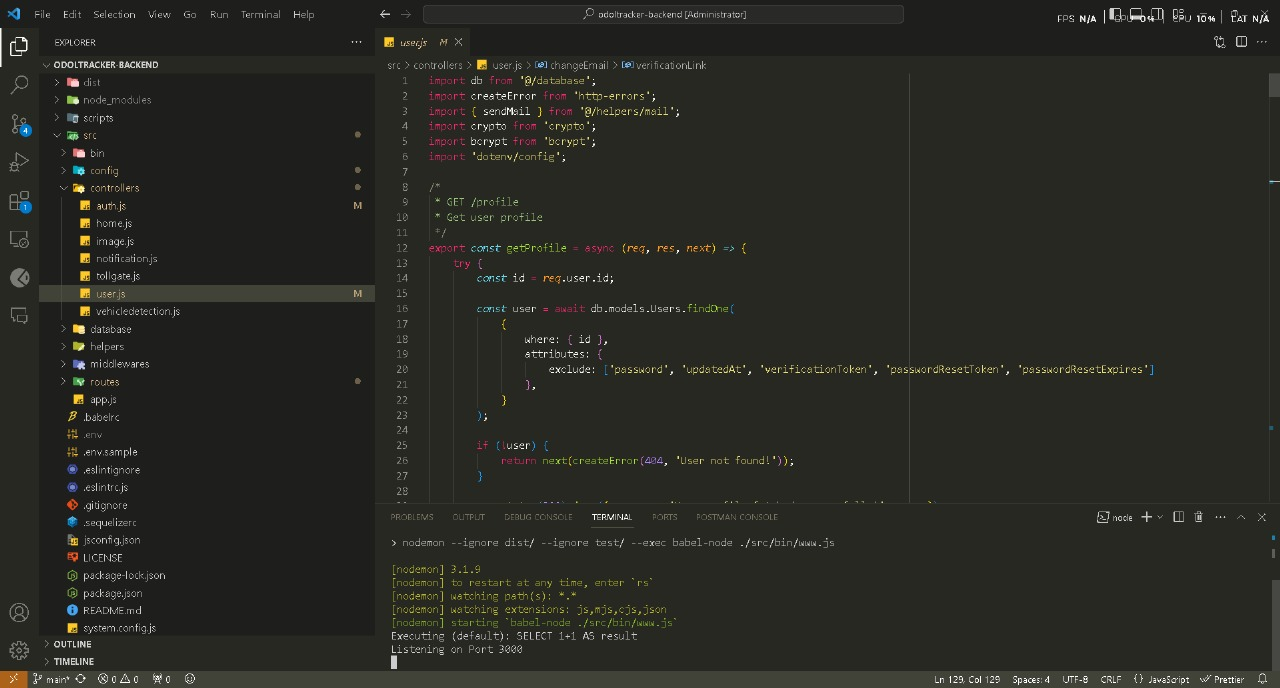
\includegraphics[scale=0.45]{gambar/bab3-implementasi-class-diagram.jpeg}

  \caption{Implementasi \emph{Class Diagram} menggunakan \emph{Express.js} dan \emph{Sequelize}}
  \label{fig:implementationclassdiagram}
\end{figure}

\subsection{\emph{Cloud}}

Pada bagian ini, dilakukan beberapa tahapan, yaitu:
\begin{enumerate}[nolistsep]
  \item Implementasi basis data di \emph{cloud}
  \item Implementasi \emph{backend} di \emph{cloud}
\end{enumerate}

\textbf{Implementasi basis data di \emph{cloud}} dilakukan setelah desain basis data selesai dilakukan. Basis data yang ada pada desain basis data akan diimplementasikan ke \emph{cloud} yang bertujuan agar basis data dapat diakses kapan saja dan di mana saja. Basis data ini diimplementasikan menggunakan \emph{cloud database} PostgreSQL dengan bantuan \emph{management tool} pgAdmin4.

\textbf{Implementasi \emph{backend} di \emph{cloud}} dilakukan setelah implementasi basis data selesai dilakukan. \emph{Backend} yang ada pada desain \emph{class diagram} akan diimplementasikan ke cloud yang bertujuan agar fungsi \emph{backend} dapat diakses kapan saja dan di mana saja. \emph{Backend} ini diimplementasikan menggunakan \emph{Virtual Private Server} dengan menggunakan \emph{cloud} \emph{platform} Biznet Gio Neo Lite. Gambar \ref{fig:implementationbackend} menunjukkan implementasi \emph{backend} yang telah dilakukan.

\begin{figure}[htbp]
  \centering

  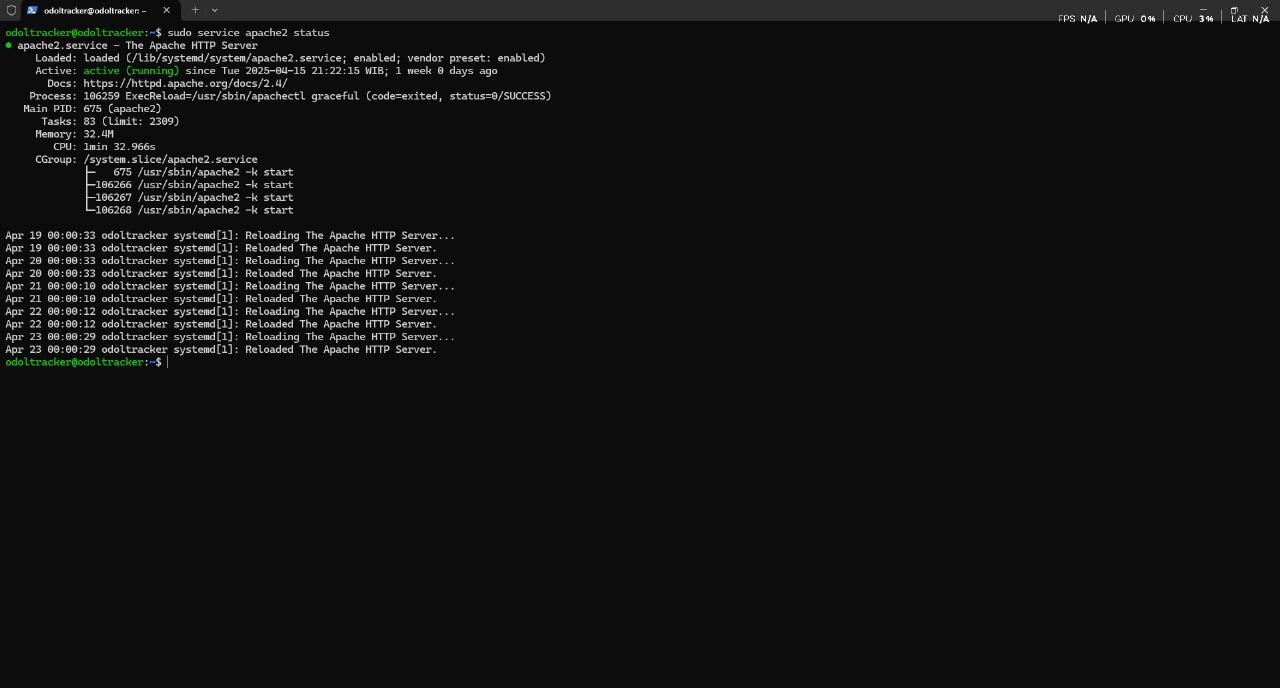
\includegraphics[scale=0.47]{gambar/bab3-implementasi-backend.jpeg}
  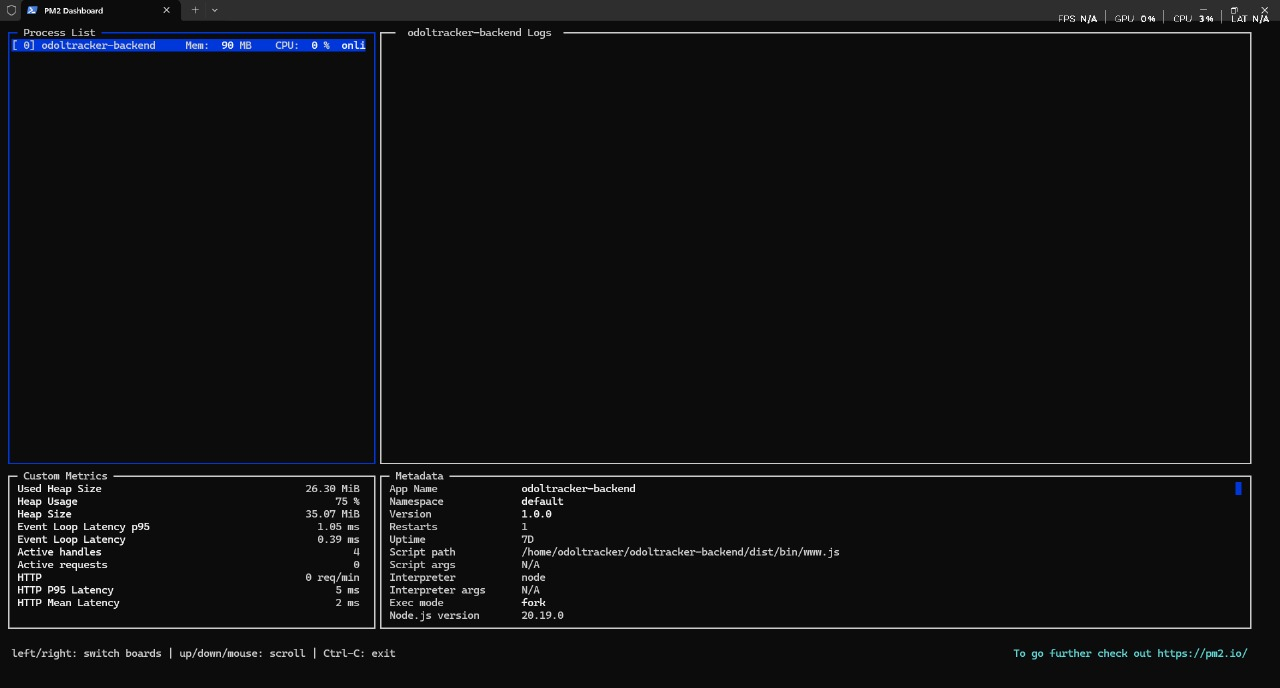
\includegraphics[scale=0.47]{gambar/bab3-implementasi-backend-2.jpeg}

  \caption{\centering Implementasi \emph{backend} di \emph{cloud}, (atas) \emph{web server backend} menggunakan Apache2, (bawah) \emph{backend} berjalan di atas \emph{process manager} PM2}
  \label{fig:implementationbackend}
\end{figure}

\subsection{\emph{Software} - Aplikasi \emph{Mobile}}

Pada bagian ini, dilakukan beberapa tahapan, yaitu:
\begin{enumerate}[nolistsep]
  \item Desain \textit{Wireframe} dan \textit{Mockup}
  \item Pembuatan \emph{prototype} aplikasi
  \item Integrasi \emph{backend} dengan aplikasi
  \item \emph{Testing} aplikasi
\end{enumerate}

\textbf{Desain \textit{Wireframe} dan \textit{Mockup}} dilakukan untuk menentukan tampilan aplikasi yang akan dibuat. Desain ini akan membantu dalam membuat aplikasi yang sesuai dengan kebutuhan pengguna. Gambar \ref{fig:wireframe} menunjukkan desain \textit{wireframe} dan \textit{mockup} yang telah dibuat.

\begin{figure}[htbp]
  \centering

  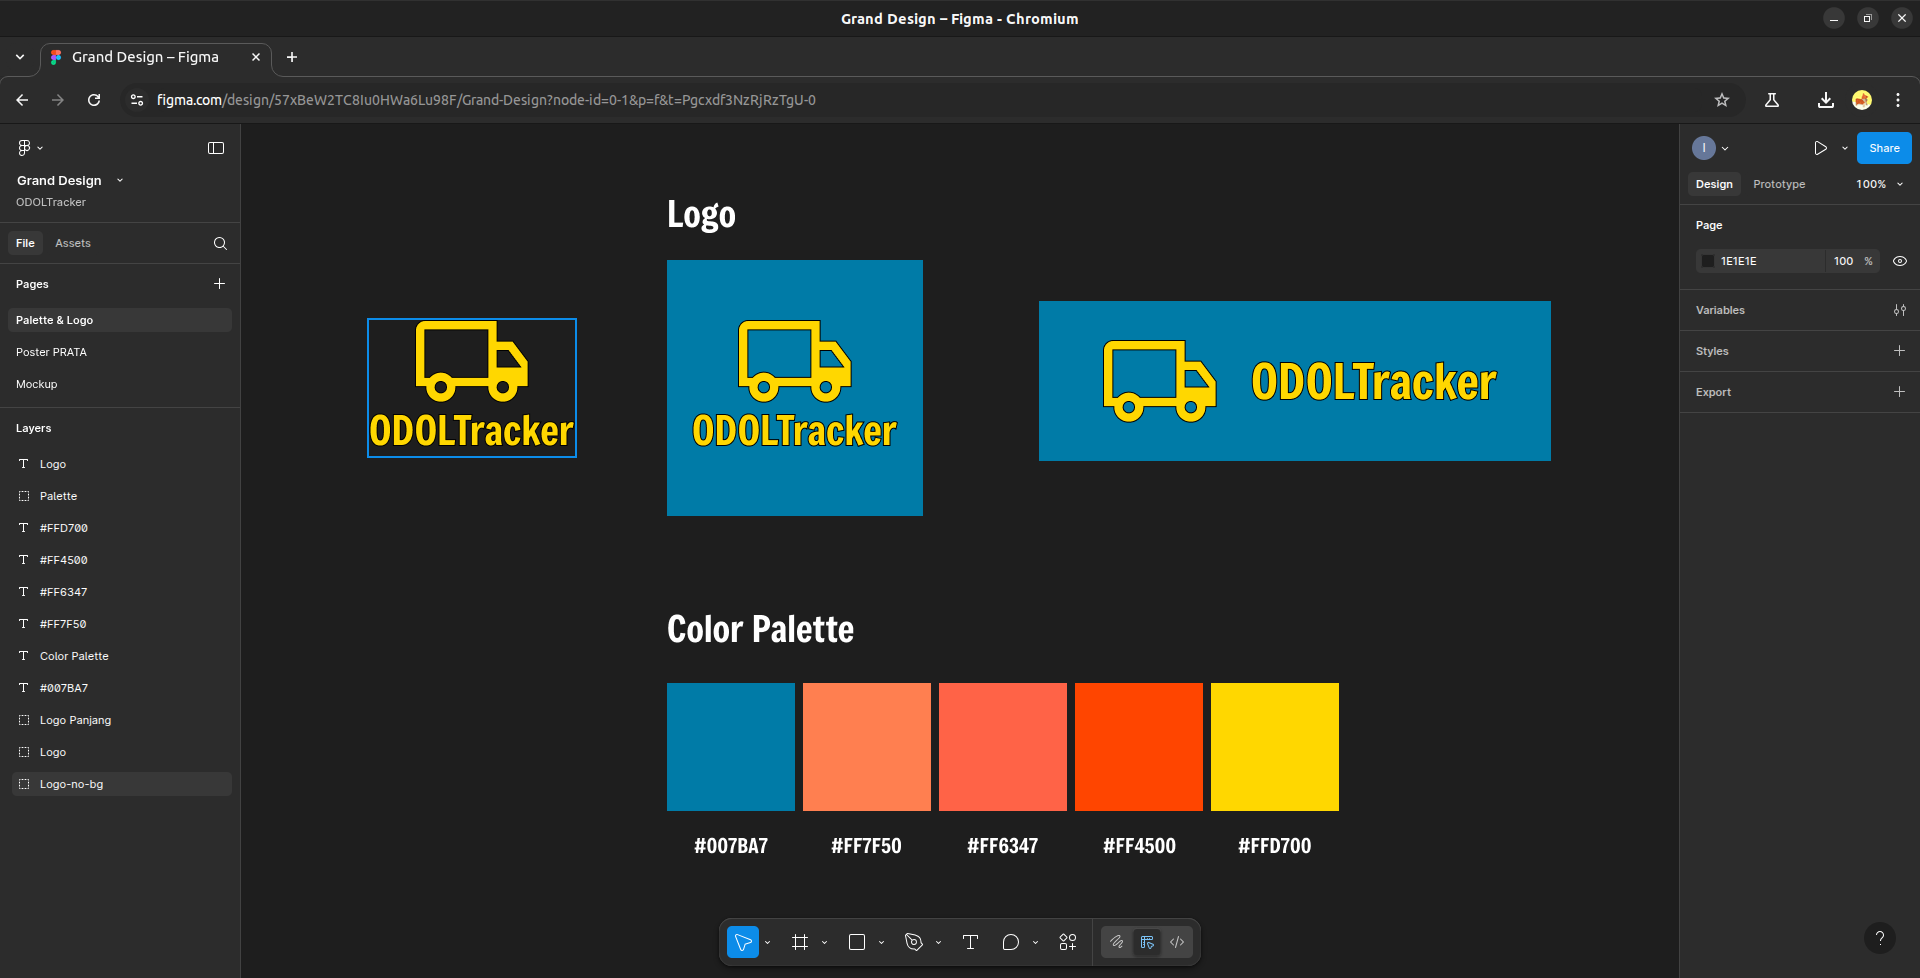
\includegraphics[scale=0.23]{gambar/bab3-color-palette.png}
  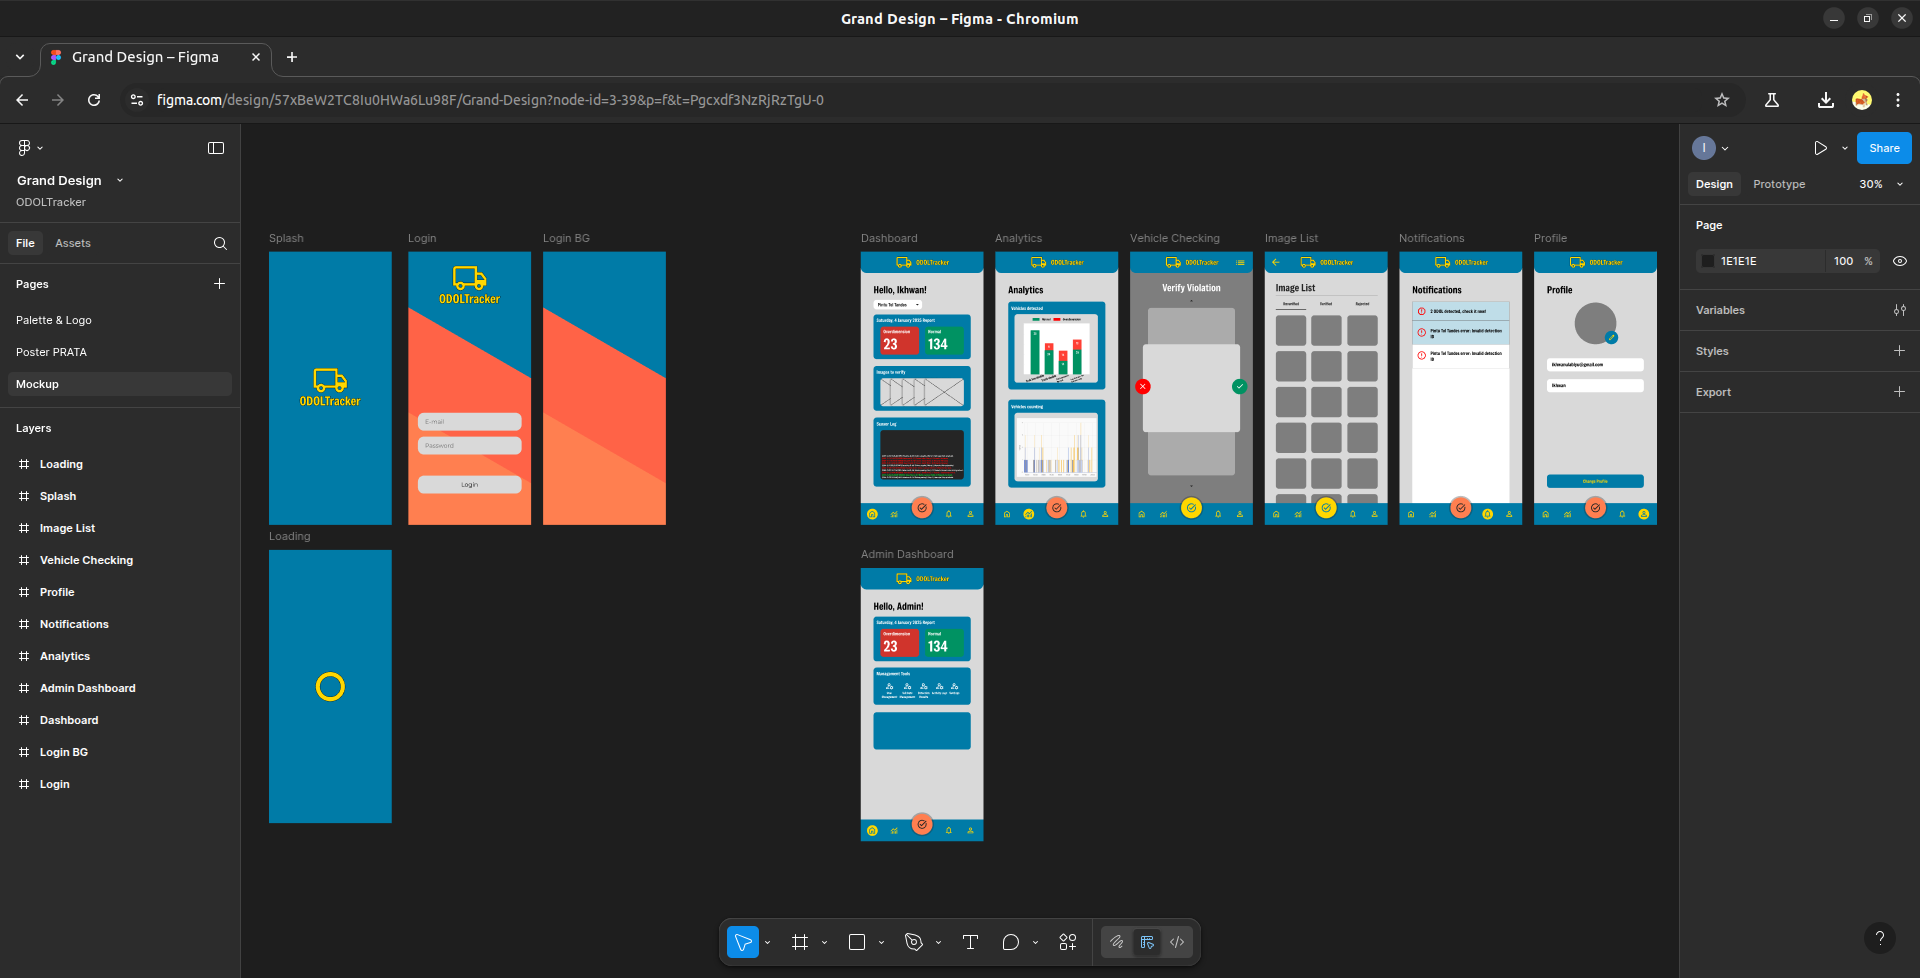
\includegraphics[scale=0.23]{gambar/bab3-mockup.png}

  \caption{\centering Desain \textit{Wireframe} dan \textit{Mockup}, (kiri) Palet Warna, (kanan) Mockup}
  \label{fig:wireframe}
\end{figure}

\textbf{Pembuatan \emph{prototype} aplikasi} dan \textbf{Integrasi \emph{backend} dengan aplikasi} dilakukan setelah desain \textit{wireframe}, \textit{mockup}, dan \emph{backend} selesai dibuat. \emph{Prototype} ini akan membantu dalam membuat aplikasi yang sesuai dengan kebutuhan pengguna. Gambar \ref{fig:prototype} menunjukkan \emph{prototype} aplikasi yang telah dibuat.

\begin{figure}[htbp]
  \centering

  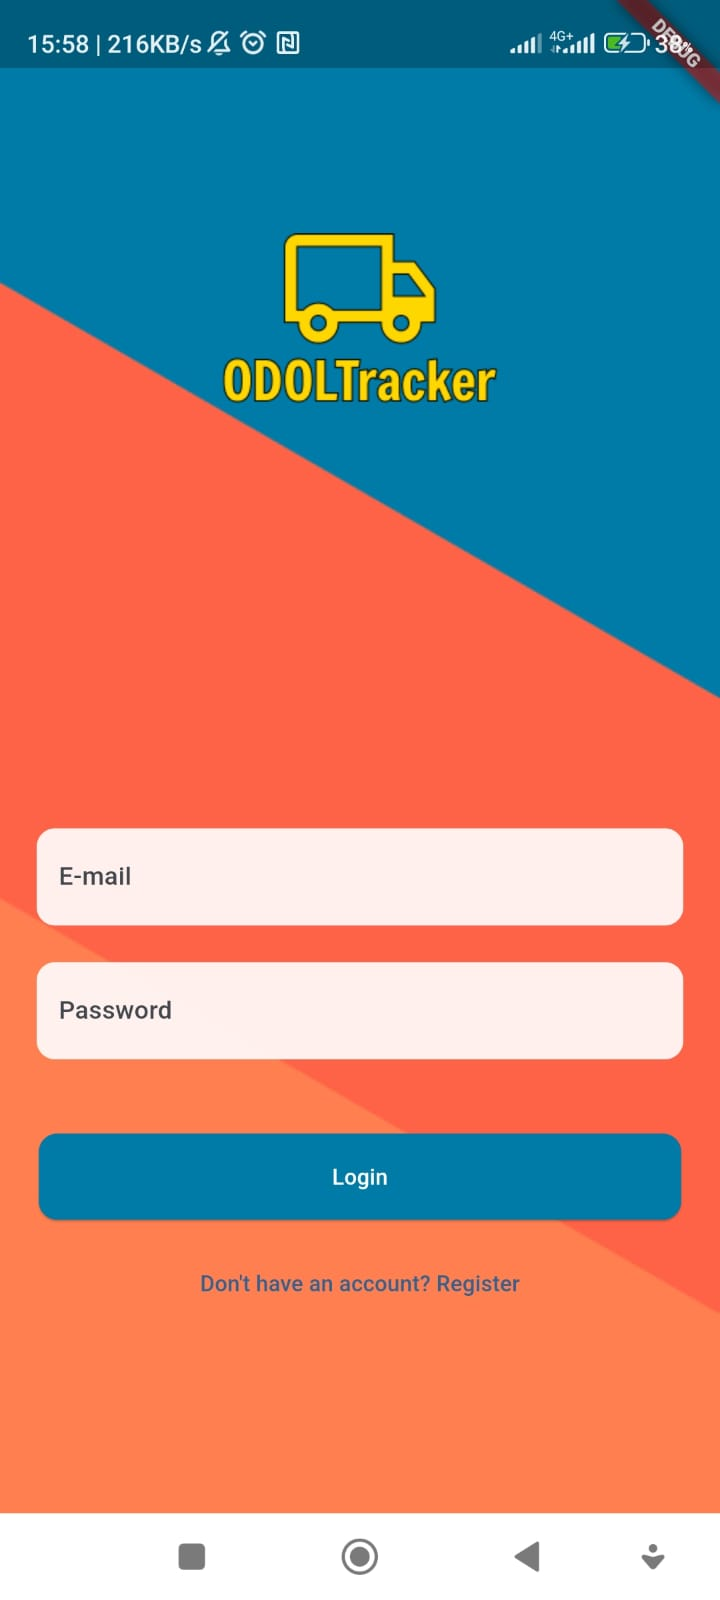
\includegraphics[scale=0.2]{gambar/bab3-login.jpeg}
  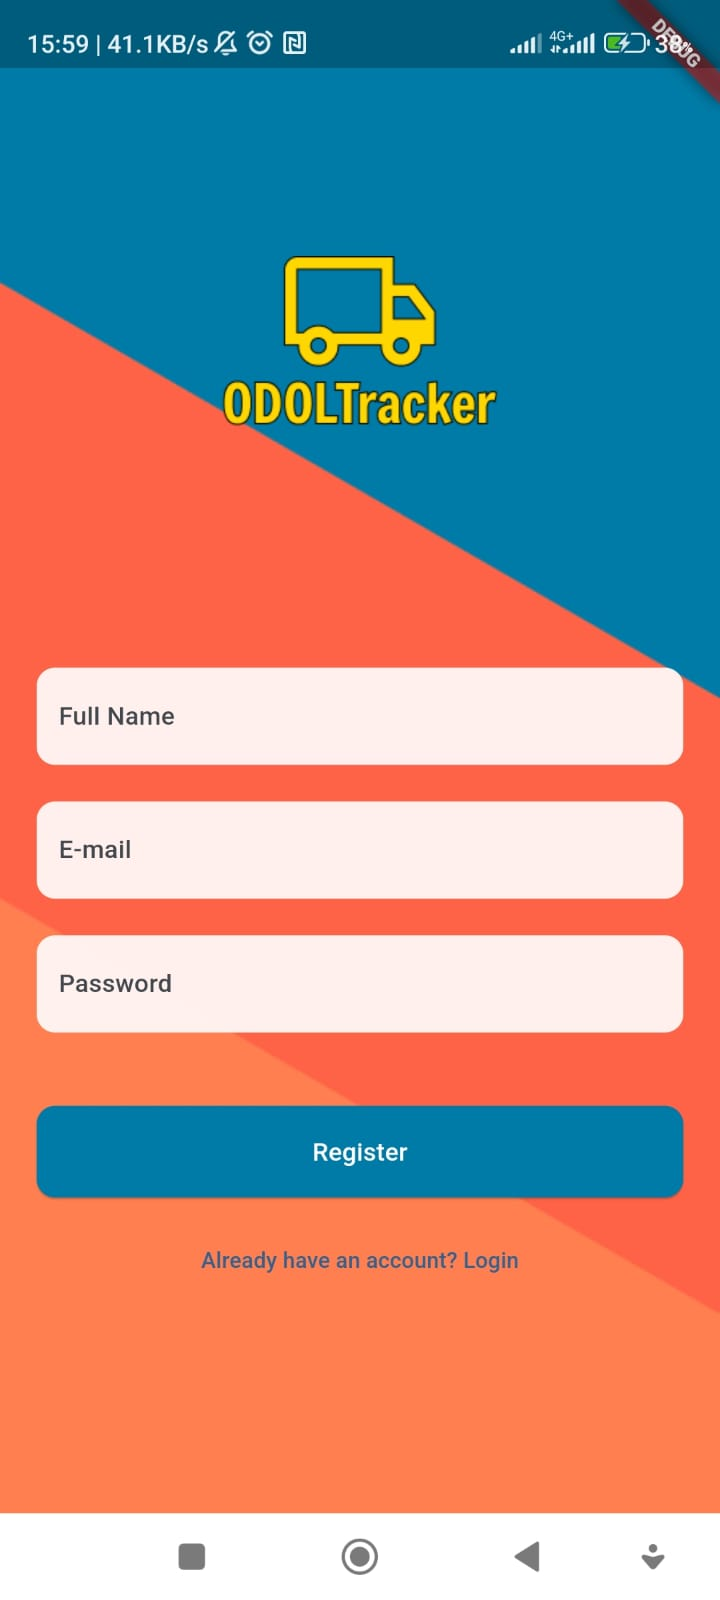
\includegraphics[scale=0.2]{gambar/bab3-register.jpeg}
  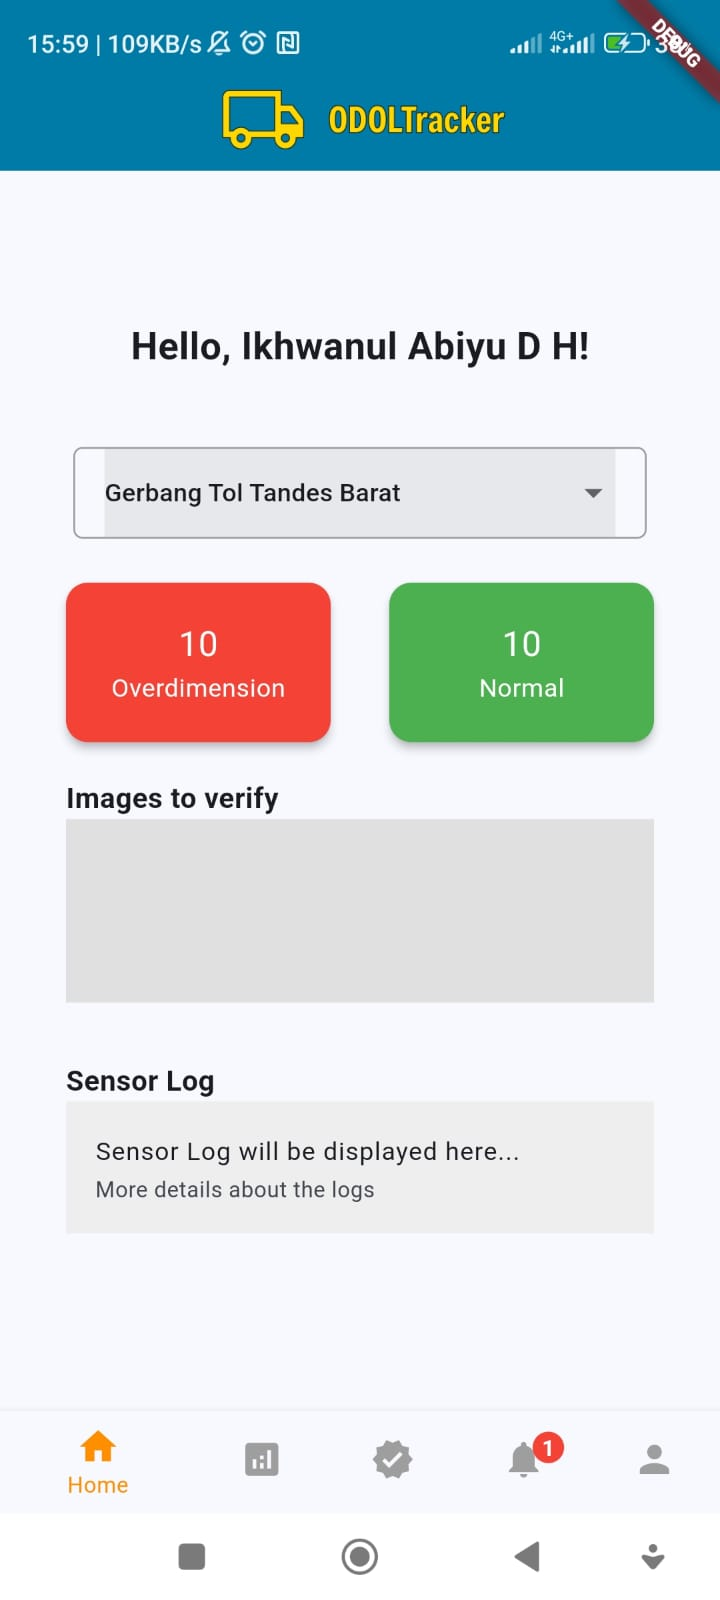
\includegraphics[scale=0.2]{gambar/bab3-homepage.jpeg}
  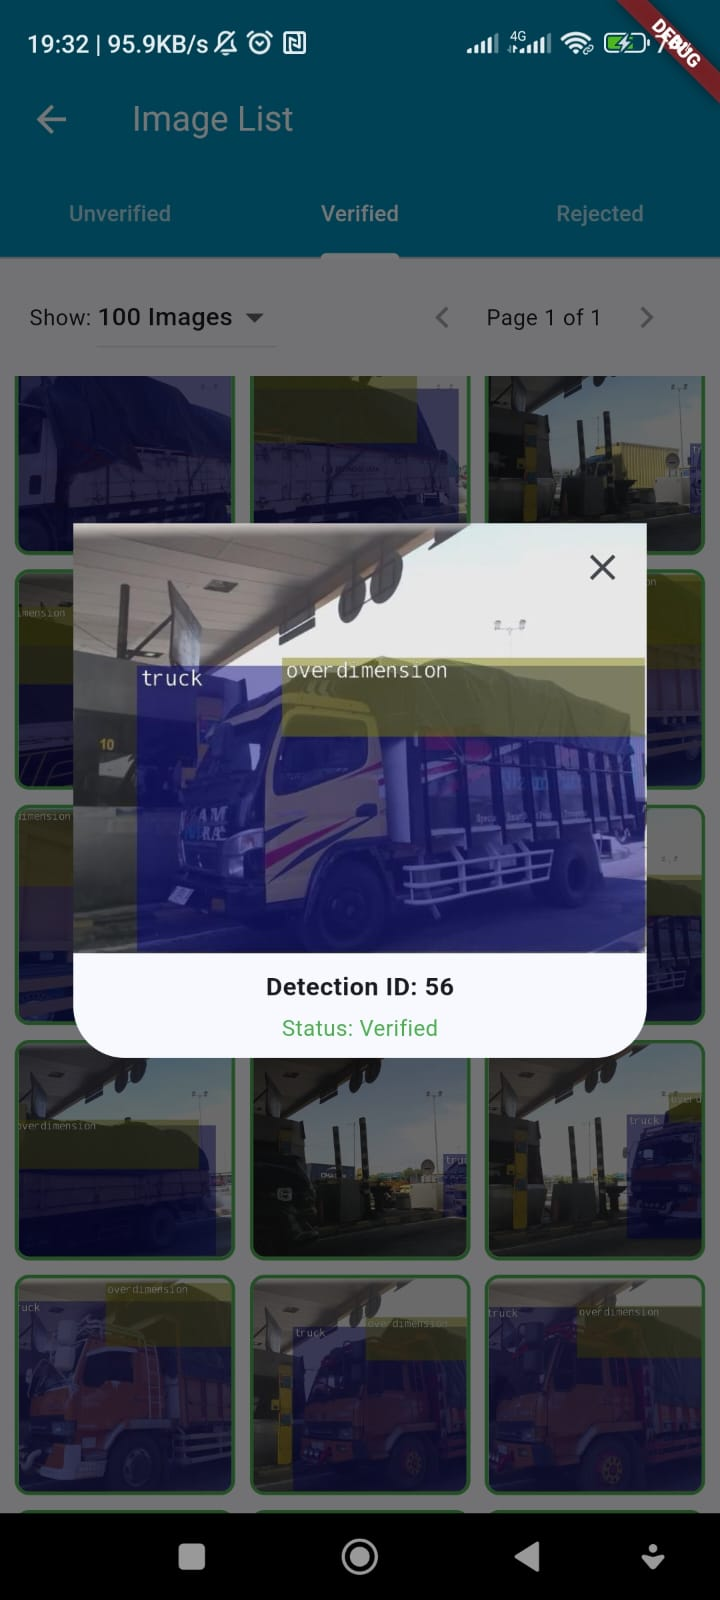
\includegraphics[scale=0.2]{gambar/bab3-contoh-verified.jpeg}


  \caption{\centering \emph{Prototype} Aplikasi (Dari kiri atas searah jarum jam: Login, Registrasi, Dashboard, Contoh Gambar \emph{Overdimension} terverifikasi)}
  \label{fig:prototype}
\end{figure}

\begin{figure}[htbp]
  \centering
  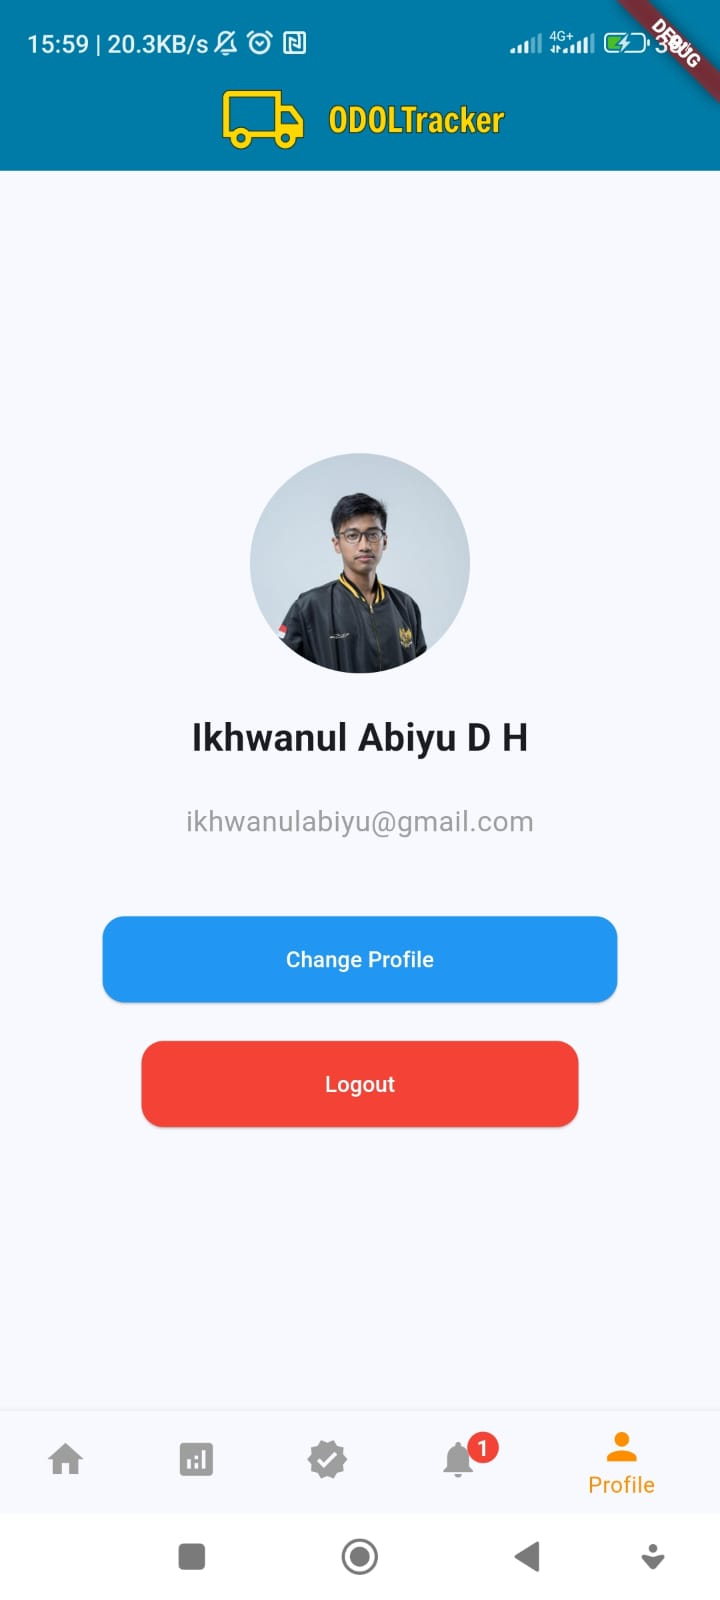
\includegraphics[scale=0.2]{gambar/bab3-profile.jpeg}
  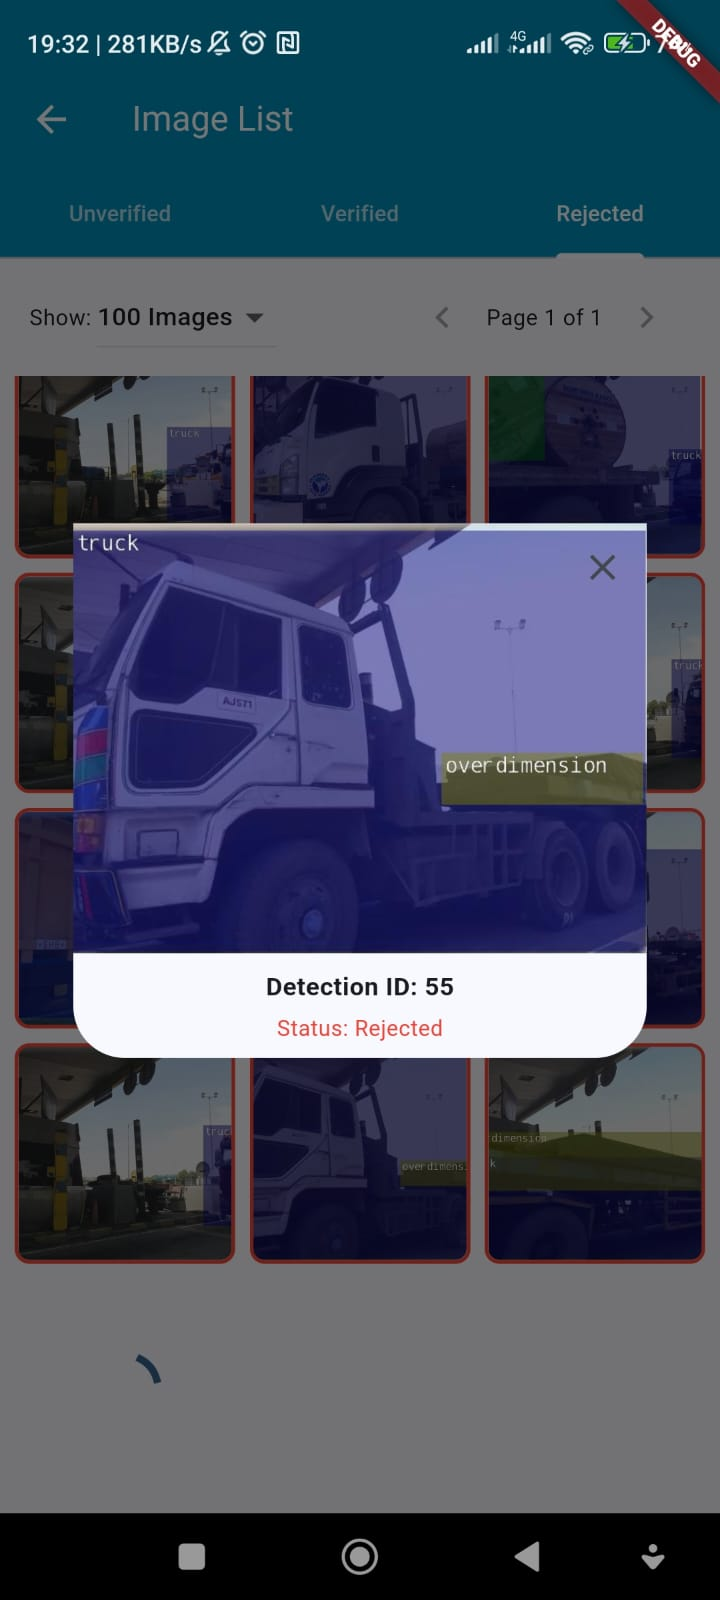
\includegraphics[scale=0.2]{gambar/bab3-contoh-rejected.jpeg}
  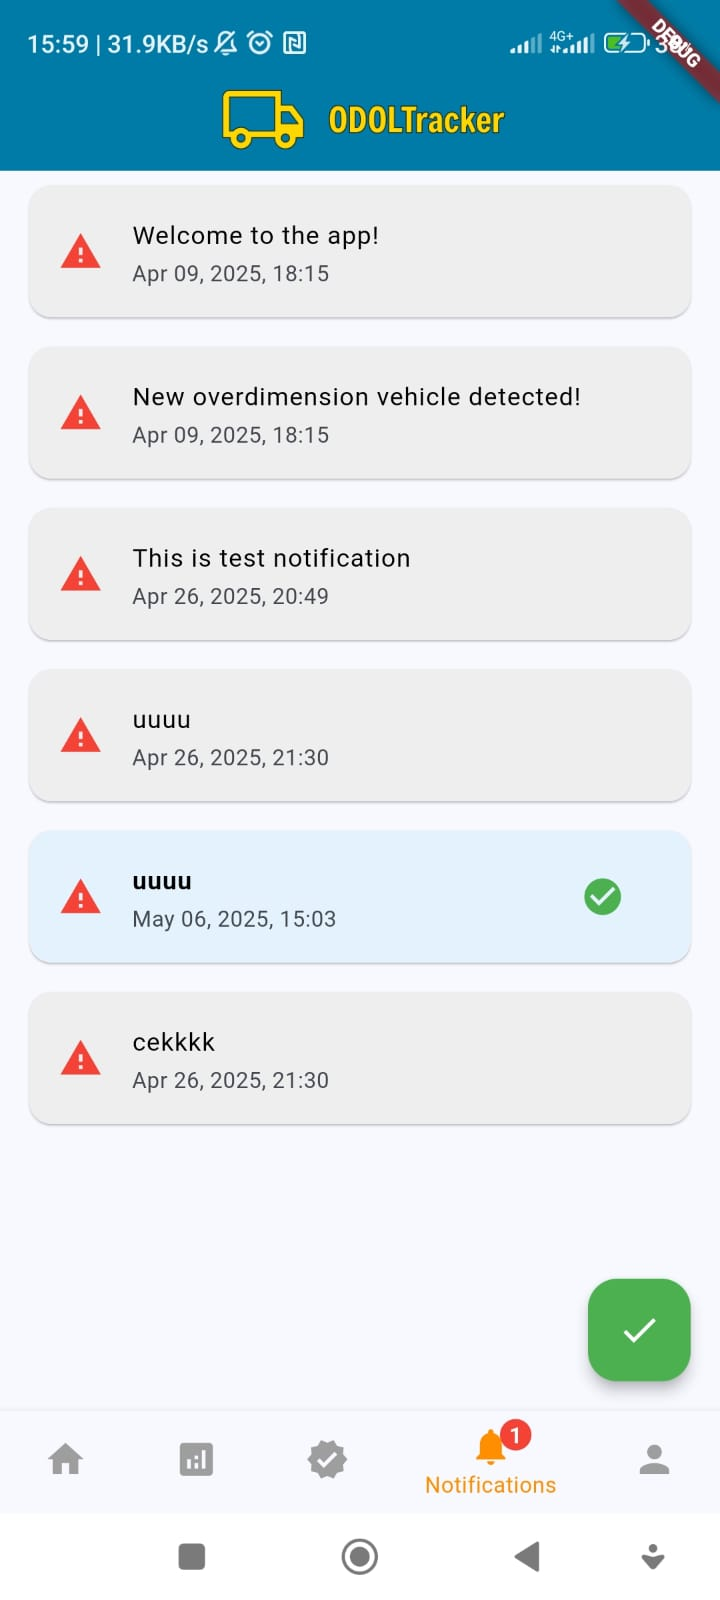
\includegraphics[scale=0.2]{gambar/bab3-notification.jpeg}
  \caption{\centering \emph{Prototype} Aplikasi (Dari kiri atas searah jarum jam: Profil, Contoh Gambar \emph{Overdimension} ditolak, Notifikasi)}
  \label{fig:profile}
\end{figure}

\textbf{\emph{Testing} aplikasi} dilakukan setelah aplikasi selesai diintegrasikan dengan \emph{backend}. \emph{Testing} ini bertujuan untuk memastikan bahwa aplikasi dapat berjalan dengan baik dan sesuai dengan kebutuhan pengguna. \emph{Testing} ini dilakukan dengan cara menguji setiap fitur yang ada pada aplikasi secara \emph{end to end}. Tabel \ref{tab:testingapp} menunjukkan hasil \emph{testing} aplikasi yang telah dilakukan.

\begin{table}[htbp]
  \centering
  \caption{Hasil pengujian fitur aplikasi}
  \label{tab:testingapp}
  \begin{tabular}{|l|l|l|}
  \hline
  \textbf{Fitur} & \textbf{Skenario} & \textbf{Status} \\
  \hline
  \multirow{2}{*}{Registrasi} & Registrasi dengan data valid & Berhasil \\
  \cline{2-3}
  & Registrasi dengan data tidak valid & Berhasil \\
  \hline
  \multirow{2}{*}{Login} & Login dengan kredensial benar & Berhasil \\
  \cline{2-3}
  & Login dengan kredensial salah & Berhasil \\
  \hline
  \multirow{2}{*}{Dashboard} & Menampilkan data pelanggaran & Berhasil \\
  \cline{2-3}
  & Memperbarui data secara otomatis & Berhasil \\
  \hline
  \multirow{2}{*}{Notifikasi} & Menerima notifikasi pelanggaran & Berhasil \\
  \cline{2-3}
  & Menampilkan riwayat notifikasi & Berhasil \\
  \hline
  \multirow{2}{*}{Profil} & Menampilkan data pengguna & Berhasil \\
  \cline{2-3}
  & Mengubah data pengguna & Berhasil \\
  \hline
  \end{tabular}
\end{table}